
%
% This draft dated January 29, 2016  [MB]
%

\documentclass[final,leqno,onefignum,onetabnum]{siamltex1213}
\usepackage{amssymb,amsmath,bm}
\usepackage{color}
\usepackage[lined,boxruled]{algorithm2e}
\usepackage{comment}
\usepackage{calrsfs}
\usepackage{amsfonts}
\usepackage{mathrsfs}
\usepackage{rotating}
\usepackage{multirow}
\DeclareMathAlphabet{\pcal}{OMS}{zplm}{m}{n}

 \newtheorem{thm}{Theorem}
% \newtheorem{lemma}{Lemma}
 \newtheorem{defn}{Definition}
 \newtheorem{prop}{Proposition}
\newtheorem{rem}{Remark}

\hoffset 0.6in

%opening
\title{Analysis of Monte Carlo accelerated iterative methods for
sparse linear systems}
\author{Michele Benzi\thanks{Department of Mathematics and Computer
Science, Emory University, Atlanta, Georgia 30322, USA
(benzi@mathcs.emory.edu). The work of this author was supported
by Department of Energy (Office of Science) grant ERKJ247.}
\and
Thomas M.~Evans\thanks{Oak Ridge National Laboratory, 1 Bethel Valley Rd., 
Oak Ridge, TN 37831, USA (evanstm@ornl.gov).}
\and Steven P. Hamilton\thanks{Oak Ridge National Laboratory, 
1 Bethel Valley Rd., Oak Ridge, TN 37831, USA (hamiltonsp@ornl.gov).}
\and 
\linebreak Massimiliano Lupo  Pasini\thanks{Department of Mathematics and Computer
Science, Emory University, Atlanta, Georgia 30322, USA (mlupopa@emory.edu).}
\and 
Stuart R.~Slattery\thanks{Oak Ridge National Laboratory,
1 Bethel Valley Rd., Oak Ridge, TN 37831, USA (slatterysr@ornl.gov).}
}
\date{}

\begin{document}
\bibliographystyle{siam}

\pagestyle{myheadings}
\markboth{{\sc M.~Benzi, T.~M.~Evans, S.~P.~Hamilton, M.~Lupo Pasini, and S.~Slattery}}
{Monte Carlo solvers for sparse linear systems}

\maketitle

\begin{abstract}
We consider hybrid deterministic-stochastic iterative algorithms for the solution
of large, sparse linear systems. Starting from a convergent splitting of the 
coefficient matrix, we analyze various types of Monte Carlo acceleration schemes
applied to the original preconditioned Richardson (stationary) iteration. These
methods are expected to have considerable potential for resiliency to faults
when implemented on massively parallel machines.

We establish sufficient conditions for the convergence of the hybrid schemes, and
we investigate different types of preconditioners including sparse approximate
inverses. Numerical experiments on linear systems arising from the discretization
of partial differential equations are presented.
\end{abstract}

\begin{keywords}
sparse linear systems, iterative methods, Richardson iteration, preconditioning,
Monte Carlo methods, sparse approximate inverses, resilience
\end{keywords}

\begin{AMS}
65C05, 65F50, 65F08, 65F10
\end{AMS}


\section{Introduction}
\label{sec:intro}

The next generation of computational science applications will require numerical
solvers that are both reliable and capable of high performance on projected exascale
platforms. In order to meet these goals, solvers must be resilient to soft and hard 
system failures, provide high concurrency on heterogeneous hardware configurations,
and retain numerical accuracy and efficiency. In this paper we focus on the
solution of large sparse systems of linear equations, for
example of the kind arising from the discretization of partial differential
rquations (PDEs).  A possible approach is to try to adapt existing solvers
(such as preconditioned Krylov subspace or multigrid methods) to the new
computational environments, and indeed several efforts are under way in this
direction; see, e.g., \cite{Agullo,FLRU15,Heroux,Rizzi,Stoyanov} and references therein. 
An alternative approach is to investigate
new algorithms that can address issues of resiliency, particularly fault
tolerance and hard processor failures, naturally. An example is provided
by the recently proposed {\em Monte Carlo Synthetic Acceleration Methods}
(MCSA), see \cite{EMSH2014,Slattery2013}. 
In these methods, an underlying (deterministic) stationary Richardson iterative
method is combined with a stochastic, Monte Carlo-based ``acceleration" scheme.
Ideally, the accelerated scheme will converge to the solution of the linear
system in far fewer (outer) iterations than the basic scheme without Monte Carlo
acceleration, with the added advantage that most of the computational effort
is now relegated to the Monte Carlo portion of the algorithm, which is 
highly parallel and offers a more straightforward path to resiliency
than standard, deterministic solvers. In addition,
a careful combination of the Richardson
and Monte Carlo parts of the algorithm allows to circumvent the well known
problem of slow Monte Carlo error reduction; see \cite{EMSH2014}.

Numerical evidence presented in \cite{EMSH2014} suggests
that MCSA can be competitive, for certain classes of problems,
with established deterministic solvers such as preconditioned 
conjugate gradients and GMRES. So far, however, no theoretical analysis
of the convergence properties of these solvers has been carried out. In
particular, it is not clear a priori whether the method, applied to a
particular linear system, will converge. 
Indeed, the convergence of the underlying preconditioned Richardson
iteration is not sufficient, in general, to guarantee the convergence
of the MCSA-accelerated iteration. In other words, it is quite possible
that the stochastic ``acceleration" part of the algorithm may actually
cause the hybrid method to diverge or stagnate.

In this paper we address this fundamental issue,
discussing both necessary and sufficient conditions for convergence.
We also discuss the choice of splitting, or preconditioner, and illustrate
our findings by means of numerical experiments. 
We do not specifically
consider in this paper the resiliency issue, which will be addressed 
elsewhere. 

The paper is organized as follows.
In Section~\ref{sec:mcls} we provide an overview of existing Monte Carlo
linear solver algorithms.
In Section~\ref{sec:convergence} we will discuss the convergence behavior
of stochastic solvers, including a discussion of classes of matrices for
which convergence can be guaranteed.
Section~\ref{sec:results} provides some numerical results illustrating
properties of the various approaches and in Section~\ref{sec:conclusion} we
give our conclusions.


\section{Stochastic linear solvers}
\label{sec:mcls}

Linear solvers based on stochastic techniques have a
long history, 
going back to the famed 1928 paper by Courant, Friedrichs, and Lewy
on finite difference schemes for PDEs \cite{CFL}. 
Many authors have considered linear solvers based on Monte Carlo
techniques, with important early contributions by
Curtiss \cite{Curtiss} and by Forsythe and Leibler \cite{FL50}. 
More recent works include \cite{AADBTW2005,Hal1994},
and \cite{DA1998}, among others.
Until recently, 
these methods have had mixed success at best,
due to their generally inferior performance when compared to state-of-the-art
deterministic solvers like multigrid or preconditioned Krylov methods.
Current interest in resilient solvers, where some performance may be
traded off for increased robustness in the presence of faults, has prompted a fresh 
look at methods incorporating Monte Carlo ideas 
\cite{EMSH2014,ESW2013,Slattery2013}.

As mentioned in \cite{DA1998}, Monte Carlo methods may be divided into two broad
classes: \textit{direct methods}, such as those described in \cite{DA1998,DVA2001}, and
\textit{iterative methods}, which refer to techniques such as those presented
in \cite{Hal1962,Hal1994}; see also \cite{EMSH2014,ESW2013}.
The first type consists of purely stochastic schemes,
therefore the resulting error with respect to the exact solution is made of
just a stochastic component. In contrast, the iterative Monte Carlo methods utilize more
traditional iterative algorithms alongside the stochastic approach,
generating two types of error: a
\textit{stochastic} one and a \textit{systematic} one. 
In practice, it may be difficult to separate the two components;
nevertheless, awareness of this intrinsic structure is useful, as it allows 
algorithm designers some flexibility in the choice of what part of the algorithm
to target for refinement (e.g., trading off convergence speed for resilience by
balancing the number of ``deterministic" outer iterations
against the number of random walks to be used within each iteration).

Consider a system of linear equations of the form
\begin{equation}
A \mathbf{x}=\mathbf{b},
\label{linsys}
\end{equation}
where $A\in \mathbb{R}^{n\times n}$ and $\mathbf{x}$, $\mathbf{b} \in
\mathbb{R}^n$.
Equation~(\ref{linsys}) can be recast as a fixed point problem:
\begin{equation}
 \mathbf{x}=H\mathbf{x}+\mathbf{f},
 \label{fixedpoint}
\end{equation}
where $H=I-A$ and $\mathbf{f}=\mathbf{b}$.
Assuming that the spectral radius $\rho(H)<1$, the solution to
\eqref{fixedpoint} can be written in terms of a power series in
$H$ (Neumann series):
\[
\mathbf{x}=\sum_{\ell=0}^\infty H^\ell\mathbf{f}.
\]
Denoting the $k$th partial sum by $\mathbf{x}^{(k)}$, the sequence of approximate solutions
$\{\mathbf{x}^{(k)}\}_{k=0}^{\infty}$ converges to the exact solution
regardless of the initial guess $\mathbf{x}_0$.

By restricting the attention to a single component of $\mathbf{x}$ we
obtain
\begin{equation}
x_i=f_i + \sum_{\ell=1}^\infty \sum_{k_1=1}^n\sum_{k_2=1}^n\cdots 
\sum_{k_{\ell}=1}^n
H_{i,k_1}H_{k_1,k_2}\cdots H_{k_{\ell-1}, k_{\ell}}f_{k_{\ell}}.
\label{forward}
\end{equation}
The last equation can be reinterpreted as the realization of an estimator
defined on a random walk.  Let us start considering a random walk whose
state space $S$ is labeled by the set of indices of the forcing term
$\mathbf{f}$:
\[
S=\{1,2,\ldots, n\} \subset \mathbb{N}.
\]
Each $i$th step of the random walk has a random variable
$k_i$ associated with it. The realization of $k_i$ represents the index of the
component of $\mathbf{f}$
which is visited in the current step of the random walk.
The transition probabilities and the selection of
the initial state of the random walk can be accomplished according to 
different modalities, leading to two distinct methods:
the \textit{forward} and \textit{adjoint} methods.
These methods are described next.

\subsection{Forward method}
\label{subsec:forward}

The general goal is to evaluate a functional as
\[
J(\mathbf{x})=\left \langle\mathbf{h},\mathbf{x}\right\rangle=\sum_{i=1}^n h_i 
x_i,
\]
where $\mathbf{h}\in \mathbb{R}^n$ is the Riesz representative in
$\mathbb{R}^n$ of the functional $J$.
Such a representative can be used to build the initial probability 
$\tilde{p}:
S\rightarrow [0,1]$ of the random walk as
\[
\tilde{p}(k_0=i)=\tilde{p}_{k_0}=\frac{\lvert h_i\rvert}{\sum_{i=1}^n 
\lvert h_i\rvert}.
\]
It is important to highlight that the role of vector $\mathbf{h}$ is
confined to the construction of the initial probability, and that $\mathbf{h}$
is not
used afterwards in the stochastic process.
A possible choice for the transition probability $P$ can be
\[
p(k_{\ell}=j \;\lvert\;k_{\ell-1}=i )=P_{ij}=\frac{\lvert 
H_{ij}\rvert}{\sum_{k=1}^n
\lvert H_{ik}\rvert}.
\]
where 
\[
p(\cdot,i):S\rightarrow [0,1], \qquad \forall i\in S
\]
and $k_{\ell}\in S$ 
represents the state reached at a generic $\ell$th step of the random walk.
A related sequence of random variables $w_{ij}$ can be defined
as
\[
w_{ij}=\frac{H_{ij}}{P_{ij}}.
\]
The probability distribution of the random variables $w_{ij}$ is represented
by the transition matrix that governs the stochastic process. The $w_{ij}$
quantities just introduced can be used to build one more sequence
of random variables.
At first we introduce quantities $W_\ell$
\[
W_{0}=\frac{h_{k_0}}{\tilde{p}_{k_0}}, \quad W_{\ell}=W_{\ell-1} 
w_{k_{\ell-1},k_{\ell}}.
\]
By introducing $\nu$ as a generic permutation that represents the realization 
of a random walk, we define
\[
X(\nu)=\sum_{\ell=0}^\infty W_{\ell} f_{k_{\ell}}
\]
as the random variable associated with a specific permutation $\nu$. 
We can thus
define the estimator $\theta$ as
\[
\theta=E[X]=\sum_{\nu}P_{\nu}X(\nu),
\]
where $\nu$ ranges over all possible realizations.
$P_{\nu}$ is the probability associated with a specific permutation of the
random walk.
It can be proved (see \cite{Hal1962} and \cite{Hal1994}) that
\[
E[W_{\ell} 
f_{k_{\ell}}]=\left\langle\mathbf{h},H^{\ell}\mathbf{f}\right\rangle, \quad 
\ell=0,1,2,\ldots
\]
and
\[
\theta=E\bigg[\sum_{\ell=0}^\infty W_{\ell} 
f_{k_{\ell}}\bigg]=\left\langle\mathbf{h},\mathbf{x}\right\rangle.
\]

A possible choice for $\mathbf{h}$ is a vector of the standard basis, 
$\mathbf{h} = \mathbf{e}_i$. This
would correspond to setting the related initial probability to a Kronecker 
delta:
\[
\tilde{p}(k_0=j)=\delta_{ij}.
\]
By doing so, we have $k_0 = i$ and 
\begin{equation}
%\theta= E\bigg[\sum_{\ell=0}^\infty W_{\ell}
%f_{k_{\ell}}\bigg]= 
\theta = x_i= 
f_i + \sum_{l=1}^\infty
\sum_{k_1=1}^{n}\sum_{k_2=1}^n\cdots \sum_{k_{\ell}=1}^n
P_{i,k_1}P_{k_1,k_2}\cdots P_{k_{\ell-1},
k_{\ell}}w_{i,k_1}w_{k_1,k_2}\cdots
w_{k_{\ell-1}, k_{\ell}}f_{k_{\ell}}.
\label{dir_mean}
\end{equation}

As regards the variance, we recall the following relation:
\begin{equation}
Var\bigg [\sum_{\ell=0}^\infty W_{\ell}
f_{k_{\ell}}\bigg]=E\bigg[\sum_{\ell=0}^\infty W_{\ell}^2
f_{k_{\ell}}^2\bigg] - \bigg (E\bigg[\sum_{\ell=0}^\infty W_{\ell}
f_{k_{\ell}}\bigg]\bigg )^2.
\label{dir_var}
\end{equation}

Hence, the variance can be computed as the difference between the second
moment of the random variable and the square of its first moment.\newline

In order to apply the Central Limit Theorem (CLT) to the estimators defined
above, we must require that
the estimators have both finite expected value and finite variance. This is
equivalent to
checking the finiteness of the expected value and second moment.
Therefore, we have to impose the following conditions:

\begin{equation}
 E\bigg[\sum_{\ell=0}^\infty W_{\ell} f_{k_{\ell}}\bigg]<\infty,
\end{equation}

\begin{equation}
 E\bigg[\sum_{\ell=0}^\infty W_{\ell}^2
f_{k_{\ell}}^2\bigg]<\infty .
\end{equation}

The forward method presented above, however, has the limitation of employing an
entire set of permutations to estimate just a single entry of
the solution at a time. Hence, in order to estimate the entire solution
vector for Eq.~\eqref{linsys}, we have to employ a separate set of
permutations for each entry in the solution vector. This limitation
can be circumvented by the adjoint method which we describe below.

\begin{rem}
It is important to note that in order to construct the random walks, 
access to the individual entries of $H$ is required. Hence, $H$ needs to be formed explicitly
and therefore must be sparse in order to have a practical algorithm.
\end{rem}

\subsection{Adjoint method}
\label{subsec:adjoint}

A second Monte Carlo method can be derived by considering the linear system
adjoint to \eqref{linsys}:
\begin{equation}
A^T\mathbf{y}=\mathbf{d},
\label{adj}
\end{equation}
where $\mathbf{y}$ and $\mathbf{d}$ are the adjoint solution and source term.
Equation \eqref{adj} can be recast in a manner similar to \eqref{fixedpoint}:
\[
\mathbf{y} = H^T \mathbf{y} + \mathbf{d}.
\]
Note that $\rho(H^T) = \rho(H) <1$, hence convergence of the Neumann series
(fixed point iteration) for (\ref{linsys}) guarantees convergence
for the adjoint system (\ref{adj}).

Exploiting the following inner product equivalence:
\[
\left\langle 
A^T\mathbf{y},\mathbf{x}\right\rangle=\left\langle\mathbf{y},A\mathbf{x} 
\right\rangle ,
\]
it follows that
\begin{equation}
\left\langle\mathbf{x},\mathbf{d}\right\rangle=\left\langle\mathbf{y},\mathbf{f}
\right\rangle.
\label{adj_relationship}
\end{equation}

By writing the Neumann series for the solution to \eqref{adj} we have:
\[
\mathbf{y}=\sum_{\ell=0}^{\infty} (H^T)^\ell \mathbf{d},
\]
and focusing on a single entry of the solution vector:
\[
y_i = d_i + \sum_{\ell=1}^{\infty}\sum_{k_1=1}^{n}\sum_{k_2=1}^n 
\cdots \sum_{k_{\ell}=1}^n H^T_{i,k_1} H^T_{k_1,k_2}\cdots 
H^T_{k_{\ell-1},k_{\ell}} d_{k_\ell}.
\]

The undetermined quantities in the dual problem \eqref{adj} are $\mathbf{y}$ 
and 
$\mathbf{d}$. Therefore, two constraints are required: the first constraint is 
Eq.~\eqref{adj_relationship} and as a second constraint we select
$\mathbf{d}$ to be one of the standard basis vectors.
Applying this choice of $\mathbf{d}$ to (\ref{adj_relationship}) we get:
\[
\left\langle\mathbf{y},\mathbf{f}\right\rangle=\left\langle\mathbf{x},\mathbf{d}
\right\rangle=x_i.
\]

In order to give a stochastic interpretation of the adjoint method similar to 
the one obtained for the forward method, we introduce the initial probability:
\[
\tilde{p}(k_0=i)=\frac{\lvert f_i\rvert}{\lVert 
\mathbf{f}\rVert_1}
\]
and the initial weight:
\[
W_0 = \lVert \mathbf{f}\rVert_1\frac{f_i}{\lvert f_i \rvert}.
\]
The transition probability is defined as 
\[
p(k_\ell = j \lvert k_{\ell-1}=i)=P_{ij}=\frac{\lvert 
H^T_{ij}\rvert}{\sum_{k=1}^n \lvert H^T_{ik}\rvert} = \frac{\lvert 
H_{ji}\rvert}{\sum_{k=1}^n \lvert H_{ki}\rvert}
\]
and the sequence of weights as follows:
\[
w_{ij}=\frac{H_{ji}}{P_{ij}}.
\]

By reformulating the fixed point scheme in its statistical interpretation, the 
following formula
holds for the estimator of the solution vector associated with the adjoint 
method: it is the vector $\boldsymbol{\theta}\in \mathbb{R}^n$ such that
\begin{equation}
%\[
\begin{array}{rl}
\theta_i& =E\bigg[\sum_{\ell=0}^\infty W_{\ell}\delta_{k_{\ell},
i}\bigg]\\
&={\displaystyle \sum_{\ell=0}^{\infty}\sum_{k_0=1}^n\sum_{k_1=1}^n\sum_{k_2=1}
^n\cdots\sum_ { k_ { \ell }=1 } ^n
f_{k_0}P_{k_0,k_1}P_{k_1,k_2}\cdots 
P_{k_{\ell-1},K_{\ell}}w_{k_0,k_1}\cdots
w_{k_{\ell-1},k_{\ell}}\delta_{k_{\ell},i}.}
\label{adj_mean}
\end{array}
%\]
\end{equation}
This estimator is known in literature as \textit{collision} estimator.

The forward method adds a contribution to the component of the solution
vector where the random walk began, based on the value of the source vector
in the state in which the walk currently resides.  The adjoint method,
on the other hand, adds a contribution to the component of the solution
vector where the random walk currently resides based on the value of the
source vector in the state in which the walk began.
The Kronecker delta at the end of the series \eqref{adj_mean} represents a 
filter, indicating
that only a subset of permutations contribute to the $j$th component
of the solution vector.

The variance is given by
\begin{equation}
Var\bigg [\sum_{\ell=0}^\infty W_{\ell}
\delta_{k_{\ell},i}\bigg]=E\bigg[\sum_{\ell=0}^\infty W_{\ell}^2
\delta_{k_{\ell},i}\bigg ] - \bigg 
(E\bigg[\sum_{\ell=0}^\infty
W_{\ell}
\delta_{k_{\ell},i}\bigg]\bigg )^2, \qquad i=1,\ldots,n
\label{adj_var}.
\end{equation}

Along the same lines as the development for the forward method, we must
impose finiteness of the expected value and second moment.
Therefore, the following
conditions must be verified:

\begin{equation}
 E\bigg[\sum_{\ell=0}^\infty W_{\ell}\delta_{k_{\ell},
i}\bigg]<\infty \qquad i=1,\ldots,n
\end{equation}
and
\begin{equation}
 E\bigg[\sum_{\ell=0}^\infty W_{\ell}^2
\delta_{k_{\ell},i}\bigg]<\infty, \qquad i=1,\ldots,n.
\end{equation}

The main advantage of this method, compared to the forward one, consists in the
fact that a single set of permutations is used to estimate the entire solution
vector.  Unless only a small portion of the problem is of interest, this
property often leads to the adjoint method being favored over the forward
method. 
 In other terms, the adjoint method should be preferred when approximating
the solution globallly over the entire computational domain, while the forward
method is especially useful when approximating the solution locally. 

In literature another estimator is employed along with the adjoint Monte Carlo
method, the so called \textit{expected value} estimator. Its
formulation is as follows: it is the vector
$\boldsymbol{\theta}\in \mathbb{R}^n$ such that
\begin{equation}
\begin{array}{rl}
\theta_i & =E\bigg[f_i + \sum_{\ell=0}^\infty
W_{\ell}H_{k_{\ell}, i}^T\bigg]\\
&=f_i 
+{\displaystyle \sum_{\ell=0}^{\infty}\sum_{k_0=1}^n\sum_{k_1=1}^n\sum_{k_2=1} ^n\cdots\sum_ 
{ k_ { \ell}=1}^n
f_{k_0}P_{k_0,k_1}P_{k_1,k_2}\cdots 
P_{k_{\ell-1},k_{\ell}}w_{k_0,k_1}\cdots
w_{k_{\ell-1},k_{\ell}}H_{k_{\ell},i}^T.}
\label{adj_mean1}
\end{array}
\end{equation}

Hence, the expected value estimator averages
the deterministic contribution of the iteration matrix over all the potential
states $j$ that might be reached from the current state $\ell$. The variance
in this case becomes:
\begin{equation}
Var\bigg [\sum_{\ell=0}^\infty W_{\ell}
H_{k_{\ell},i}^T\bigg]=E\bigg[\sum_{\ell=0}^\infty W_{\ell}^2
{H_{k_{\ell},i}^T}^T\bigg ] - \bigg 
(E\bigg[\sum_{\ell=0}^\infty
W_{\ell}
H_{k_{\ell},i}^T\bigg]\bigg )^2, \qquad i=1,\ldots,n
\label{adj_var1}.
\end{equation}

\subsection{Hybrid stochastic/deterministic methods}

The direct methods described in Sections~\ref{subsec:forward} and
\ref{subsec:adjoint} suffer from a slow rate of convergence due to the
$\frac{1}{\sqrt{N}}$ behavior dictated by the central limit theorem ($N$ here
is the number of random walks used to estimate the solution).  Furthermore,
when the spectral radius of the iteration matrix is close to unity, each
individual random walk may require a large number of transitions to
approximate the corresponding components in the Neumann series.
To offset the slow convergence of the central limit theorem, schemes have
been proposed which combine traditional fixed point iterative methods with
the stochastic solvers.  The first such method, due to Halton, was termed
the Sequential Monte Carlo (SMC) method, and can be written as follows.

\begin{algorithm}[H]
 %\SetAlgoLined
 %\BlankLine
 \LinesNumbered
 \KwData{$H$, $\mathbf{b}$, $\mathbf{x}_0$}
 \KwResult{$\mathbf{x}_{num}$}
 $l=0$\;
 \While{not reached convergence}{
  $\mathbf{r}^{l}=\mathbf{b}-A\mathbf{x}^{l}$\;
  $\delta \mathbf{x}^{l+1}\approx(I-H)^{-1}\mathbf{r}^{l}$; \qquad 
\text \% {Computed via Standard MC}
  $\mathbf{x}^{l+1}=\mathbf{x}^{l}+\delta \mathbf{x}^{l+1}$\;
  $l=l+1$\;
 }
 $\mathbf{x}_{num}=\mathbf{x}^{l+1}$\;
 \caption{Sequential Monte Carlo}
\end{algorithm}


The Monte Carlo linear solver method is used to compute the update $\delta
\mathbf{x}^{l}$.  This algorithm is equivalent to a Richardson iteration
accelerated by a correction obtained by approximately solving the error-residual
equation
\begin{equation}
(I - H)\delta \mathbf{x}^{l+1} = \mathbf{r}^{l}.
\label{eq:corr}
\end{equation}
If this equation were to be solved exactly, the corresponding approximation
$\mathbf{x}^{l+1}=\mathbf{x}^{l}+\delta \mathbf{x}^{l+1}$ would be the exact
solution to the linear system. This is of course impractical, since solving
(\ref{eq:corr}) is equivalent to solving the original linear system
(\ref{linsys}). Instead, the correction is obtained by
solving (\ref{eq:corr}) only approximately, using a Monte Carlo method.
Because Monte Carlo is only applied within a single iteration, the central
limit theorem is only applicable within that iteration rather than to
the overall convergence behavior of the algorithm. This allows a trade-off
between the amount of time and effort spent on the inner (stochastic) and
outer (deterministic) iterations, which can take account the competing goal
of reliability and rapid convergence.

A further extension of Halton's method, termed
\textit{Monte Carlo Synthetic Acceleration} (MCSA), has been recently
introduced in \cite{ESW2013} and \cite{EMSH2014}.  The MCSA algorithm can be 
written as:

\begin{algorithm}[H]
\LinesNumbered
 \KwData{$H$, $\mathbf{b}$, $\mathbf{x}_0$}
 \KwResult{$\mathbf{x}_{num}$}
 $l=0$\;
 \While{not reached convergence}{
  $\mathbf{x}^{l+\frac{1}{2}}=H\mathbf{x}^l+\mathbf{b}$\;
  $\mathbf{r}^{l+\frac{1}{2}}=\mathbf{b}-A\mathbf{x}^{l+\frac{1}{2}}$\;
 $\delta\mathbf{x}^{l+\frac{1}{2}}\approx(I-H)^{-1}\mathbf{r}^{l+\frac{1}{2}}$; 
\qquad
\% \text{Computed via Standard MC}
  $\mathbf{x}^{l+1}=\mathbf{x}^{l+\frac{1}{2}}+\delta
\mathbf{x}^{l+\frac{1}{2}}$\;
 $l=l+1$\;
 }
 $\mathbf{x}_{num}=\mathbf{x}^{l+1}$\;
 \caption{Monte Carlo Synthetic Acceleration}
\end{algorithm}

As with SMC, a Monte Carlo linear solver is used to compute the updating
contribution $\delta \mathbf{x}^{l+\frac{1}{2}}$.  In this approach, an
extra step of Richardson iteration is added to smooth out
some of the high-frequency noise introduced by the Monte Carlo process.
This way, the deterministic and stochastic components of the algorithm
act in a complementary fashion.

Obviously, a minimum requirement is that the linear system can be written
in the form (\ref{fixedpoint}) with $\rho(H) < 1$. This is typically achieved by
preconditioning. That is, we find an invertible matrix $P$ such that $H = I - P^{-1}A$
satisfies $\rho(H) < 1$, and we apply the method to the fixed point problem
(\ref{fixedpoint}) where $H = I - P^{-1}A$ and $\mathbf{f} = P^{-1}\mathbf{b}$. In
other words, the underlying deterministic iteration is a preconditioned
Richardson iteration. Various choices of the preconditioner are possible;
a detailed discussion of this issue is deferred until Section \ref{sec:prec}.
Here we note only that because we need explicit 
knowledge of the entries of $H$, not all preconditioning choices are
viable; in particular, $P$ needs to be such that $H = I - P^{-1}A$ retains
a high degree of sparsity. Unless otherwise specified, below we
assume that the transformation of the original linear system (\ref{linsys})
to the fixed point form (\ref{fixedpoint}) with $\rho(H)<1$ has already
been carried out.

\section{Convergence behavior of stochastic methods}
\label{sec:convergence}

Interestingly,
the convergence requirements imposed by the Monte Carlo estimator and
the corresponding variance can be reformulated in a purely deterministic
setting.
For instance, the condition of finiteness of the expected value turns out to 
be equivalent to requiring
\begin{equation}
 \rho(H)<1
 \label{rho_h},
\end{equation}
where $H$ is the iteration matrix of the fixed point scheme.
Indeed, we can see from (\ref{dir_mean}) and (\ref{adj_mean}) that the
expected value is expressed in terms of
power series of $H$, and the condition $\rho(H)<1$ 
is a necessary and sufficient condition for the Neumann series to
converge.

Next, we address the finiteness requirement for the second moment.
Equations \eqref{dir_var} and \eqref{adj_var}
for
the forward and the adjoint method, respectively, show that the second
moment can be reinterpreted as a power series with respect to the matrices
defined as follows:
\[
 \hat{H}_{ij}=\frac{H_{ij}^2}{P_{ij}} \quad \text{- Forward Method}
\]
and
\[
 \hat{H}_{ij}=\frac{H_{ji}^2}{P_{ij}} \quad \text{- Adjoint Method}.
\]
In order for the corresponding power series to
converge, we must require
\begin{equation}
 \rho(\hat{H})<1.
 \label{rho_star}
\end{equation}
Hence, condition \eqref{rho_h} is required for a generic fixed point scheme to
reach convergence, whereas the extra condition \eqref{rho_star} is typical of
the stochastic schemes studied in this work.
Moreover, since the finiteness of the variance automatically entails the 
finiteness of the expected value, we can state that \eqref{rho_star} 
implicitly entails \eqref{rho_h}, whereas the converse is not true in 
general.

\subsection{Necessary and sufficient conditions}

Here we report some results presented in 
\cite{Srin2010} and \cite{MASC2013},
concerning necessary conditions and sufficient conditions for convergence.
In particular, these papers discuss suitable choices for constructing the
transition probability matrix, $P$.

The construction of the transition probability must obviously satisfy the following 
constraints (called \textit{transition conditions}):
\[
\begin{cases}
  P_{ij}\ge 0 \\
 \sum_{j=1}^N P_{ij}= 1 \,.
\end{cases}
\]
One additional requirement relates the sparsity pattern of $H$ to that
of the transition probabilities:
\begin{align*}
& \text{Forward Method:} \quad H_{ij}\ne 0 \Rightarrow P_{ij}\ne 0, \\ &
\text{Adjoint Method:} \quad H_{ji}\ne 0 \Rightarrow P_{ij}\ne 0.
\end{align*} 
The following auxiliary result can be found in \cite{MASC2013}.

\begin{lemma}
 Consider a generic vector 
$\mathbf{g}=(g_1,g_2,\ldots,g_N)^T$ where at least 
one element is
nonzero, $g_k\ne0$ for some $k\in\{1,\ldots,N\}$. %$N$ represents the 
%arbitrary length of the vector $\mathbf{g}$. 
Then, the following statements hold:
\begin{enumerate}
 \item[(i)] for any probability distribution vector 
$\boldsymbol{\beta}=(\beta_1,\beta_2,\ldots,
\beta_N)^T$ satisfying the
transition conditions, $\displaystyle
\sum_{k=1}^N\frac{g_k^2}{\beta_k}\ge \bigg(\sum_{k=1}^N 
\lvert g_k\rvert\bigg)^2$; moreover, the lower bound is attained for
the probability vector defined by $\displaystyle \beta_k=\frac{\lvert
g_k\rvert}{\sum_{k=1}^N \lvert g_k\rvert}$;
\item[(ii)] there always exists a probability vector 
$\boldsymbol{\beta}$ such that $\displaystyle
\sum_{k=1}^N\frac{g_k^2}{\beta_k}\ge c$, for all 
$c>1$.
\end{enumerate}
\label{lemma1}
\end{lemma}

Consider now a generic realization of a random walk, truncated at a certain $k$th step:
\[
% \gamma_k:\; r_0\rightarrow r_1 \rightarrow r_2 \rightarrow \cdots \rightarrow r_k,
 \nu_k:\; r_0\rightarrow r_1 \rightarrow r_2 \rightarrow \cdots \rightarrow r_k,
\]
and the corresponding statistical estimator associated with the Forward Monte 
Carlo method:
\[
% X(\gamma_k)=\frac{H_{r_0,r_1}H_{r_1,r_2}\cdots
 X(\nu_k)=\frac{H_{r_0,r_1}H_{r_1,r_2}\cdots
H_{r_{k-1},r_k}}{P_{r_0,r_1}P_{r_1,r_2}\cdots P_{r_{k-1},r_k}}f_{r_k}.
\]
Then, the following result holds (see \cite{MASC2013}).
\begin{thm}\textit{(Forward method version)}
Let $H\in \mathbb{R}^{n\times n}$ be such that $\lVert H\rVert_{\infty}<1$.
%Consider $\nu_k$ as the realization of a random walk $\gamma$ truncated at the
Consider $\nu_k$ as the realization of a random walk $\nu$ truncated at the
$k$th step. Then,
there always exists a
transition matrix $P$ such that
$Var\Big(X(\nu_k)\Big)\rightarrow 0$ and
$Var\Big(\sum_{\nu}X(\nu_k)\Big)$ is bounded as $k\rightarrow \infty$.
\label{for_thm}
\end{thm}

If we introduce the estimator associated with the Adjoint Monte Carlo:
\[
% X(\gamma_k)=\frac{H^T_{r_0,r_1}H^T_{r_1,r_2}\cdots
 X(\nu_k)=\frac{H^T_{r_0,r_1}H^T_{r_1,r_2}\cdots
H^T_{r_{k-1},r_k}}{P_{r_0,r_1}P_{r_1,r_2}\cdots
P_{r_{k-1},r_k}}\text{sign}(f_{r_0})\lVert \mathbf{f}\rVert_1,
\]
then we can state a
theorem analogous to \ref{for_thm} (see \cite{MASC2013}).

\begin{thm}\textit{(Adjoint method version)}
 Let $H\in \mathbb{R}^{n\times n}$ with $\lVert H\rVert_{1}<1$.
%Consider $\nu_k$ as the realization of a random walk $\gamma$ truncated at the
Consider $\nu_k$ as the realization of a random walk $\nu$ truncated at the
$k$th step. Then,
there always exists a
transition matrix $P$ such that
$Var\Big(X(\nu_k)\Big)\rightarrow 0$ and
$Var\Big(\sum_{\nu}X(\nu_k)\Big)$ is bounded as $k\rightarrow \infty$.
\label{adj_thm}
\end{thm}

These results represent sufficient (but not necessary) conditions
for the convergence
of the forward and adjoint Monte Carlo and can be easily verified if $H$ is explicitly
available.
However, in many cases the conditions $\lVert H\rVert_{\infty}<1$ or
$\lVert H\rVert_1<1$ may be too restrictive.

The connection between Lemma \ref{lemma1} and Theorems \ref{for_thm}-\ref{adj_thm}
will be explained in 
the next section, dedicated to the definition of transition probabilities.


\subsection{Construction of transition probabilities}

The way the transition probability is defined has a significant impact
on the properties of the resulting algorithm, and in many circumstances the
choice can make the difference between convergence or divergence of the stochastic
scheme.  Two main approaches have been considered in the literature:
\textit{uniform probabilities} and \textit{weighted probabilities}.
We discuss these next.

\subsubsection{Uniform probabilities}

With this approach, the transition matrix $P$ is such that all the 
transitions corresponding to each row have equal probability of occurring:
\[
\text{Forward}:\;P_{ij}=
\begin{cases}
0 \quad \quad \quad \qquad \qquad \qquad \text{if}\quad H_{ij}=0, \\
\frac{1}{\#(\text{non-zeros in row $i$ of $H$)}} \quad \text{if} \quad H_{ij}\ne 0;
\end{cases}\quad
\]
\[
\text{Adjoint}:\;P_{ij}=
\begin{cases}
0 \quad \quad \quad \qquad \qquad \qquad \text{if}\quad H_{ji}=0, \\
\frac{1}{\#(\text{non-zeros in column $i$ of $H$)}} \quad \text{if} \quad H_{ji}\ne 0.
\end{cases}
\]
The Monte Carlo approach resorting to this definition of the transition matrix,
in accordance to \cite{AADBTW2005}, is called \textit{Uniform Monte Carlo} (UM).

\subsubsection{Weighted probabilities}

An alternative definition of transition matrices aims to associate nonzero 
probability to the nonzero entries of $H$ accordingly to their magnitude. For 
instance, we may employ the following definition:
\[
\text{Forward}: \;
p(k_i=j \;\lvert\;k_{i-1}=i )=P_{ij}=\frac{\lvert
H_{ij}\rvert^p}{\sum_{k=1}^n
\lvert H_{ik}\rvert^p,}
\]
and
\[
\text{Adjoint}: \;
p(k_i=j \;\lvert\;k_{i-1}=i )=P_{ij}=\frac{\lvert
H_{ji}\rvert^p}{\sum_{k=1}^n
\lvert H_{ki}\rvert^p} \,,
\]
where $p\in \mathbb{N}$.
The case $p=1$ is called
\textit{Monte Carlo Almost Optimal} (MAO).
The reason for the ``almost optimal'' designation can be understood looking 
at
Lemma~\ref{lemma1}, as the quantity
%$\displaystyle \sum_{k=1}^N\frac{\mathbf{g}_k^2}{\boldsymbol{\beta}_k}$
$\sum_{k=1}^N\frac{g_k^2}{\beta_k}$
is minimized when the probability vector is
defined as $\displaystyle \beta_k=\frac{\lvert 
g_k\rvert}{\sum_{k=1}^N \lvert
g_k\rvert}$. Indeed, Lemma~\ref{lemma1} implies that the almost optimal probability 
minimizes the
$\infty$-norm of $\hat{H}$ for the forward method and the $1$-norm of $\hat{H}$
for the adjoint method, since the role of $\mathbf{g}$ in Lemma~\ref{lemma1} is played 
by the rows of $H$ in the former case and by the columns of $H$ in the latter one. 
This observation provides us with easily computable upper bounds for 
$\rho(\hat{H})$.

\subsection{Classes of matrices with guaranteed convergence}

On the one hand, sufficient conditions for
convergence of Monte Carlo linear solvers are very restrictive; see, e.g.,
\cite{Srin2010} and \cite{MASC2013}. On the other hand, the necessary and 
sufficient 
condition in \cite{MASC2013} requires knowledge of $\rho(\hat{H})$, which 
is not readily available. Note that explicit computation of $\rho(\hat{H})$
is quite expensive, comparable to the cost of solving the original linear system.
While ensuring that $\rho(H)<1$ (by means with appropriate preconditioning)
is in many cases possible, guaranteeing that $\rho(\hat{H})<1$ is generally
much more problematic.

Here we identify matrix types for which both conditions can be satisfied
by an appropriate choice of splitting, so that convergence of the Monte Carlo scheme
is guaranteed.

%\subsubsection{Strictly Diagonally Dominant}
\subsubsection{SDD matrices}
\label{sec:sdd}

One of these categories is represented by strictly diagonally dominant 
(SDD) matrices. We investigate under which conditions diagonal preconditioning
is enough to ensure convergence.
We recall the following definitions.

\begin{defn}
 A matrix $A\in\mathbb{R}^{n\times n}$ is strictly diagonally dominant 
by rows if
 \begin{equation}
    \lvert a_{ij}\rvert>\sum_{\substack{i=1\\ i\ne j}}^{n}\lvert
a_{ij}\rvert .
\label{sddr}
 \end{equation}
\end{defn}

\begin{defn}
 A matrix $A\in\mathbb{R}^{n\times n}$ is strictly diagonally dominant
by columns if $A^T$ is strictly diagonally dominant by rows, i.e., 
 \begin{equation}
    \lvert a_{ij}\rvert>\sum_{\substack{j=1\\ j\ne i}}^{n}\lvert
a_{ij}\rvert .
\label{sddc}
 \end{equation}
\end{defn}

Suppose $A$ is SDD by rows. Then we can apply left diagonal (Jacobi) preconditioning, 
obtaining an iteration matrix $H=I-P^{-1}A$ such that $\lVert H 
\rVert_{\infty}<1$.
Introducing a MAO transition probability for the forward method: 
\[
 P_{ij}=\frac{\lvert H_{ij}\rvert}{\sum_{k=1}^n\lvert H_{ik}\rvert} 
\]
we have that the entries of $\hat{H}$ are defined as follows:
\[
 \hat{H}_{ij}=\frac{H^2_{ij}}{P_{ij}}=\lvert H_{ij}\rvert\bigg
(\sum_{k=1}^n\lvert
H_{ik}\rvert\bigg ).
\]
Consequently,
\[
 \sum_{j=1}^n\lvert \hat{H}_{ij} \rvert = \sum_{j=1}^n \hat{H}_{ij} =\bigg
(\sum_{j=1}^n \lvert H_{ij}\rvert\bigg )\bigg (\sum_{k=1}^n\lvert
H_{ik}\rvert\bigg ) =\bigg
(\sum_{j=1}^n \lvert H_{ij}\rvert\bigg ) ^2 <1, \qquad \forall i=1,\cdots, n.
\]
This implies that $\rho(\hat{H})\le \lVert
\hat{H}\rVert_{\infty}<1$, guaranteeing the forward Monte Carlo converges.
However, nothing can be said {\em a priori}
about the convergence of the adjoint method.

On the other hand, if \eqref{sddc} holds, we can apply right diagonal 
(Jacobi) preconditioning, which
results in an iteration matrix $H=I-AP^{-1}$ such that $\lVert H 
\rVert_{1}<1$.
In this case, by a similar reasoning we
conclude that the adjoint method converges, owing to $\lVert
\hat{H}\rVert_1<1$; however,
nothing can be said \textit{a priori} about the forward method.

Finally, it is clear that if $A$ is SDD by rows {\em and} by columns, then 
a (left or right) diagonal preconditioning will result in the convergence
of both the forward and the adjoint Monte Carlo schemes.

\subsubsection{GDD matrices}
\label{sec:gdd}

Another class of matrices for which the convergence of
MC solvers is ensured is that of generalized diagonally
dominant (GDD) matrices. We recall the following definition.

\begin{defn}
A square matrix $A\in\mathbb{C}^{n\times n}$ is said to be {\em generalized
diagonally dominant} if
\[
 \lvert a_{ii}\rvert d_i \ge \sum_{\substack{j=1\\j\ne i}}^n \lvert
a_{ij}\rvert
d_j, \quad i=1,\ldots,n,
\]
for some positive vector $\mathbf{d}=(d_1,\ldots,d_n)^T$.
\end{defn}

Note that this means that there exists a diagonal matrix  $\Delta$
such that $A\Delta$ is SDD.
A proper subclass of the class of GDD matrices is represented
by the nonsingular $M$-matrices.
Recall that $A$ is a nonsingular $M$-matrix if it is of the form
$A=r I - B$ where $B$ is nonnegative and $r>\rho(B)$.
It can be shown (see, e.g., \cite{BP1979}) that  a matrix
$A\in\mathbb{R}^{n\times n}$ is a nonsingular $M$-matrix if and only
if there exists a positive diagonal matrix $\Delta$ such that
$A\Delta$ is SDD by rows. Clearly, every 
nonsingular $M$-matrix is GDD. 

It is well known (see, e.g., \cite{Ax1994}) that the classical
Jacobi, Block Jacobi and Gauss--Seidel splittings are
convergent if $A$ is a nonsingular $M$-matrix.
However, this is not enough to ensure the
convergence of MC schemes based on the corresponding fixed point
(preconditioned Richardson) iteration, since in general
we cannot expect that $\rho(\hat{H})<1$. 

Nevertheless, if $A$ is an $M$-matrix there exist efficient methods
to determine a diagonal scaling of $A$ so that the resulting matrix
is SDD by rows. Note that the scaled matrix is still an $M$-matrix, 
therefore applying left Jacobi preconditioning to this matrix will
guarantee that both $\rho(H)<1$ and $\rho(\hat{H})<1$.

In \cite{Li2002}, the author presents a procedure to determine
whether a given matrix $A\in\mathbb{C}^{n\times n}$
is GDD (in which case the diagonal scaling that
makes $A$ GDD is produced), or not.
The algorithm can be described as follows.

\begin{algorithm}[H]
\LinesNumbered
 \KwData{matrix $A$, $a_{ii}\ne 0$, $i=1,\ldots, n$}
 \KwResult{$d_i$, $i=1,\ldots,n$}
 
 Compute $\displaystyle S_{i}=\sum_{\substack{j=1 \\ j\ne i}}^n\lvert
a_{ij}\rvert$,
$i=1,\ldots,n$\\
Set $t=0$\\ 
\For{$i=1,\ldots, n$}{
\If{$\lvert a_{ii}\rvert>S_i$}{$t=t+1$}
}
\uIf{$t=0$}{print ``A is not GDD"}
\uElseIf{$t=n$}{print ``A is GDD"}
\Else{
\For{$i=1,\ldots, n$}{$d_{i}=\frac{S_i+\varepsilon}{\lvert
a_{ii}\rvert+\varepsilon} \quad
\varepsilon>0,\quad j=1,\ldots,n$\\
$a_{ji}=a_{ji}\cdot d_i$}
Go to step 1
}
 \caption{Algorithm to determine whether a matrix is GDD}
\end{algorithm}

This procedure, which in practice converges very fast, turns a generalized 
diagonally dominant matrix (in particular, a nonsingular $M$-matrix) into a
strictly diagonally dominant matrix by rows. By replacing
$\displaystyle S_{i}=\sum^{n}_{\substack{j=1 \\ j\ne i}}\lvert a_{ij}\rvert$
at step 1 with
$\displaystyle S_{j}=\sum^{n}_{\substack{i=1 \\ i\ne j}}\lvert a_{ij}\rvert$
and by replacing
$a_{ji}=a_{ji}\cdot d_i$ with $a_{ji}=a_{ji}\cdot d_j$, we obtain the algorithm
that turns a GDD matrix into a matrix that is SDD by columns.

Once we have applied this transformation to the original matrix $A$
the Monte Carlo scheme combined with diagonal preconditioning
is ensured to converge.

\subsubsection{Block diagonally dominant matrices}
\label{sec:bdd}

In this section we analyze situations in which block diagonal preconditioning
can produce a convergent Monte Carlo linear solver.
Assume that $A$ has been partitioned into $p\times p$ block form, and that 
each diagonal block has size $n_i$ with $n_1 +\cdots +n_p=n$. Assume further
that each diagonal block $A_{ii}$ is nonsingular.
The iteration
matrix $H\in\mathbb{R}^{n\times n}$ resulting from a block diagonal left
preconditioning is
\[
 H=\begin{bmatrix}0_{n_1\times n_1} & -A_{11}^{-1}A_{12} & \cdots &
\cdots & -A_{11}^{-1}A_{1p} \\
-A_{22}^{-1}A_{21} & 0_{n_2\times n_2} & -A_{22}^{-1}A_{23} &
\cdots & -A_{22}^{-1}A_{2p}\\
\vdots & \vdots & \ddots & \vdots & \vdots\\
\vdots & \vdots & \vdots &\ddots & \vdots \\
-A_{pp}^{-1}A_{p1} &  \cdots & \cdots&
-A_{pp}^{-1}A_{p,p-1} & 0_{n_p \times n_p}
\end{bmatrix}.
\]

Below, we denote with ``$i|m$" the 
modulo operation applied to the integers $i$ and $m$. The 
symbol ``$\lfloor \cdot \rfloor$" stands for the floor function, as usual.

Consider first the forward method. Assuming (for ease of notation)
that all the blocks have the same size $m=n/p$,
the entries of the MAO transition probability matrix become:
\[
 P_{ij}=\frac{\lvert H_{ij} \rvert}{\sum_{k=1}^n\lvert H_{ik}
\rvert}=\frac{\bigg \lvert \bigg ([A_{\lfloor
\frac{i}{m}\rfloor \lfloor 
\frac{i}{m}\rfloor}]^{-1} A_{\lfloor \frac{i}{m}\rfloor \lfloor
\frac{j}{m}\rfloor}\bigg )_{i|m,j|m}\bigg
\rvert}{\displaystyle \sum_{\substack{k=1\\k\ne i}}^n\bigg \lvert \bigg
([A_{\lfloor
\frac{i}{m}\rfloor \lfloor
\frac{i}{m}\rfloor}]^{-1} A_{\lfloor \frac{i}{m}\rfloor \lfloor
\frac{k}{m}\rfloor}\bigg )_{i|m,k|m}\bigg \rvert}.
\]
Consequently, the entries of $\hat{H}$ are given by
\[
\begin{array}{rl}
\hat{H}_{ij} & = \lvert H_{ij}\rvert\bigg(\sum_{k=1}^n\lvert H_{ik}\rvert\bigg)\\
& =
\bigg \lvert \bigg ([A_{\lfloor \frac{i}{m}\rfloor \lfloor
\frac{i}{m}\rfloor}]^{-1} A_{\lfloor \frac{i}{m}\rfloor \lfloor
\frac{j}{m}\rfloor}\bigg )_{i|m,j|m}\bigg
\rvert
{\displaystyle
\sum_{\substack{k=1\\k\ne i}}^n\bigg \lvert \bigg ([A_{\lfloor
\frac{i}{m}\rfloor \lfloor
\frac{i}{m}\rfloor}]^{-1} A_{\lfloor \frac{i}{m}\rfloor \lfloor
\frac{k}{m}\rfloor}\bigg )_{i|m,k|m}\bigg \rvert.
}
\end{array}
\]
Computing the sum over a generic row of $\hat{H}$, we obtain 
\[
 \sum_{j=1}^n \lvert \hat{H}_{ij}\rvert=\sum_{j=1}^n \hat{H}_{ij} =
 \bigg ( \sum_{\substack{j=1\\j\ne i}}^n\bigg \lvert \bigg ([A_{\lfloor
\frac{i}{m}\rfloor \lfloor
\frac{i}{m}\rfloor}]^{-1} A_{\lfloor \frac{i}{m}\rfloor \lfloor
\frac{j}{m}\rfloor}\bigg )_{i|m,j|m}\bigg \rvert \bigg ) ^2.
\]
Consider now the quantity $\lVert \hat{H}\rVert_{\infty}$. Clearly,
\[
 \lVert \hat{H}\rVert_{\infty}<1 \Leftrightarrow \sum_{\substack{j=1\\j\ne
i}}^n\bigg \lvert \bigg ([A_{\lfloor
\frac{i}{m}\rfloor \lfloor
\frac{i}{m}\rfloor}]^{-1} A_{\lfloor \frac{i}{m}\rfloor \lfloor
\frac{j}{m}\rfloor}\bigg )_{i|m,j|m}\bigg \rvert <1, \qquad \forall
i=1,\ldots,n.
\]
 A sufficient condition for this to happen is that
 \begin{equation}
  \sum_{\substack{k=1\\k\ne h}}^p \lVert A_{hh}^{-1}A_{hk}\rVert_{\infty}<1,
    \label{block_cs}\qquad \forall h=1,\ldots,p.
 \end{equation}
Introducing the matrix $\tilde{H}\in \mathbb{R}^{p\times p}$ defined as
\[
 \tilde{H}=\begin{bmatrix}0 & \lVert A_{11}^{-1}A_{12}\rVert_{\infty} &
\cdots &
\cdots & \lVert A_{11}^{-1}A_{1p}\rVert_{\infty} \\
\lVert A_{22}^{-1}A_{21}\rVert_{\infty} & 0 & \lVert
A_{22}^{-1}A_{23}\rVert_{\infty} &
\dots & \lVert A_{22}^{-1}A_{2p}\rVert_{\infty} \\
\vdots & \vdots & \ddots & \vdots & \vdots\\
\vdots & \vdots & \vdots &\ddots & \vdots \\
\lVert A_{pp}^{-1}A_{p1}\rVert_{\infty} &  \cdots & \cdots&
\lVert A_{pp}^{-1}A_{p,p-1}\rVert_{\infty} & 0
\end{bmatrix}
\]
we can formulate a
sufficient condition on the convergence of the forward Monte
Carlo scheme:
\begin{equation}
 \lVert \tilde{H} \rVert_{\infty}<1 \Rightarrow \lVert \hat{H}
\rVert_{\infty}<1.
\end{equation}
Note that (\ref{block_cs}) also implies that $\|H\|_{\infty} < 1$. 

We now turn our attention to the adjoint method.
Analogously to the forward method, we can define
\[
(\hat{H})^T_{ij} = \lvert H^T_{ij}\rvert\bigg(\sum_{k=1}^n\lvert
H^T_{ik}\rvert\bigg) = \lvert H_{ji}\rvert\bigg(\sum_{k=1}^n\lvert
H_{ki}\rvert\bigg).
\]
This allows us to formulate a sufficient condition for the convergence of 
the adjoint Monte Carlo method with block diagonal preconditioning.
Letting
\[
  \tilde{H}=\begin{bmatrix}0 & \lVert A_{11}^{-1}A_{12}\rVert_{1} & \cdots
&
\cdots & \lVert A_{11}^{-1}A_{1p}\rVert_{1} \\
\lVert A_{22}^{-1}A_{21}\rVert_{1} & 0 & \lVert
A_{22}^{-1}A_{23}\rVert_{1} &
\cdots & \lVert A_{22}^{-1}A_{2p}\rVert_{1} \\
\vdots & \vdots & \ddots & \vdots & \vdots\\
\vdots & \vdots & \vdots &\ddots & \vdots \\
\lVert A_{pp}^{-1}A_{p1}\rVert_{1} &  \cdots & \cdots&
\lVert A_{pp}^{-1}A_{p,p-1}\rVert_{1} & 0
\end{bmatrix},
\]
a sufficient condition is that $\lVert \tilde{H} \rVert_{1}<1$, i.e.,
 \begin{equation}
  \sum_{\substack{h=1\\h\ne k}}^p \lVert A_{hh}^{-1}A_{hk}\rVert_1<1,
    \label{block_cs_2}\qquad \forall k=1,\ldots,p.
 \end{equation}
Again, this condition also implies that $\|H\|_1 < 1$.

We say that $A$ is {\em strictly block diagonally dominant by rows (columns) 
with respect to a given block partition}
if condition (\ref{block_cs}) (respectively, (\ref{block_cs_2})) is satisfied 
relative to that particular block partition.
Note that a matrix may be strictly block diagonally dominant with
respect to one partition and not to another.
We note that these definitions of block diagonal dominance are different from 
those found in, e.g., \cite{FV62}, and they are easier to check in practice
since they do not require computing the 2-norm of the blocks of $H$.

\subsection{Adaptive methods} \label{sec:adapt}

In formulas (\ref{dir_mean}) and (\ref{adj_mean}), the estimation of the
solution to
the linear system (\ref{linsys}) involves infinite sums, which in actual
computation have to be truncated. In the following we discuss criteria
to decide the number of steps to be taken in
a single random walk as well as the number of random walks that
need to be performed at each Richardson iteration.

\subsubsection{History length}

We first consider criteria to terminate an individual random walk, effectively
deciding how many terms of the Neumann series will be considered.
One possibility is to set a predetermined history length, at which point all
histories are terminated.  This approach, however, presents two difficulties.
First, it is difficult to determine a priori how many steps on average will be
necessary to achieve a specified tolerance.  Second, due to the stochastic
nature of the random walks, some histories will retain important information
longer than others.  Truncating histories at a predetermined step runs the
risk of either prematurely truncating important histories, leading to larger
errors, or continuing unimportant histories longer than necessary,
leading to computational inefficiency.

Our goal is to apply a cutoff via an automatic procedure, without requiring
any user intervention. We would like to determine
an integer $m$ such that
\[
\begin{array}{rl}
\tilde{\theta}&=E\bigg[\sum_{\ell=0}^m W_{\ell}
f_{k_{\ell}}\bigg]\\
& = f_i + {\displaystyle \sum_{\ell=1}^m
\sum_{k_1=1}^{n}\sum_{k_2=1}^n\cdots \sum_{k_{\ell}=1}^n
P_{i,k_1}P_{k_1,k_2}\cdots P_{k_{\ell-1},
k_{\ell}}w_{k_0,k_1}w_{k_1,k_2}\cdots
w_{k_{\ell-1}, k_{\ell}} f_{k_{\ell}}
}
\end{array}
\]
and %$\tilde{\boldsymbol{\theta}}\in \mathbb{R}^n$ s.t.
\[
\begin{array}{rl}
\tilde{\theta}_i&=E\bigg[\sum_{\ell=0}^m W_{\ell}\delta_{k_{\ell},
j}\bigg]\\
& ={\displaystyle \sum_{\ell=0}^{m}\sum_{k_1}^n\sum_{k_2}^n\cdots\sum_{k_{\ell}}^n
f_{k_0}P_{k_0,k_1}P_{k_1,k_2}\cdots 
P_{k_{\ell-1},K_{\ell}}w_{k_0,k_1}\cdots
w_{k_{\ell-1},k_{\ell}}\delta_{k_{\ell},i}
}
\end{array}
\]
are good approximations of (\ref{dir_mean}) and (\ref{adj_mean}), respectively.

In \cite{Slattery2013} a criterion was given which is applicable to both 
forward and adjoint methods. It requires to set up a relative weight cutoff 
threshold $W_c$ and to look for a step $m$ such that
\begin{equation}
W_m \le W_c W_0 \,.
\label{cutoff}
\end{equation}
In (\ref{cutoff}), $W_0$ is the value of the weight at the initial step of the random walk
and $W_m$ is the value of the weight after $m$ steps.
We will adopt a similar strategy in this work.

\subsubsection{Number of random walks}

We now consider the selection of the number of random walks that should be
performed to achieve a given accuracy. Unlike the termination of histories,
this is a subject that has not been discussed in the Monte Carlo linear
solver literature, as all previous studies have considered the simulation
of a prescribed number of histories.

The expression for the variance of the forward method is given by
formula (\ref{dir_var}).
In this context, a reasonable criterion to determine the number $\tilde{N}_i$
of random walks to be run is to set a threshold $\varepsilon_1$ and determine
$\tilde{N}_i$ such that
\begin{equation}
\frac{\sqrt{Var[\theta_i]}}{\lvert
E[\theta_i]\rvert}<\varepsilon_1, \quad i=1,\ldots,n.
\label{forward_adapt}
\end{equation}
The dependence of $Var[\theta_i]$ and $E[\theta_i]$ on $\tilde{N}_i$
is due to the fact that
$\theta_i$ is estimated by performing a fixed  number of histories.
Therefore, we are controlling the relative standard deviation, requiring it not
to be too large. In other words, we are aiming for an approximate solution in which 
the uncertainty factor is small relative to the expected value.
This simple adaptive approach can be applied for the estimation of each
component $x_i$. Hence, a different number of histories may be employed to
compute different entries of the solution vector.

As concerns the adjoint method, the estimation of the variance is 
given in formula \eqref{adj_var}.
A possible criterion for the adaptive selection of the number $\tilde{N}$ of random
walk, in this situation, is that it satisfies the condition
\begin{equation}
\frac{\lVert
\boldsymbol{\sigma}^{\tilde{N}}\rVert_1}{\lVert
\mathbf{x}\rVert_1}<\varepsilon_1,
\label{adjoint_adapt}
\end{equation}
where $\boldsymbol{\sigma}$ is a vector whose entries are
$\sigma^{\tilde{N}}_i=Var[\theta_i]$ and $\mathbf{x}$ is a vector whose entries 
are $x_i = E[\theta_i]$.

The criteria introduced above can be exploited to build
an a posteriori adaptive algorithm, capable of identifying the minimal value of
$\tilde{N}$ that verifies \eqref{forward_adapt} or \eqref{adjoint_adapt},
respectively.
Algorithms \ref{alg:adaptive_for} and \ref{alg:adaptive_adj} describe
the Monte Carlo approaches with the adaptive criteria.

\begin{algorithm}[H]
\LinesNumbered
 \KwData{$N$, $\varepsilon_1$}
 \KwResult{$\tilde{N}_i$, $\sigma_i$, $x_i$}
 \For{$i=1,\ldots,n$}
 {
 $\tilde{N}_i=N$\;
 compute $x_i$\;
 compute $\sigma_i$\;
 \While{$\frac{\sigma_i}{\lvert
x_i\rvert}<\varepsilon_1$}{
\vspace{0.1cm}
  $\tilde{N}=\tilde{N}+N$\;
  compute $x_i$\;
  compute $\sigma_i$\;
 }
 }
 \caption{A posteriori adaptive Forward Monte Carlo \label{alg:adaptive_for}}
\end{algorithm}

\begin{algorithm}[H]
\LinesNumbered
 \KwData{$N$, $\varepsilon_1$}
 \KwResult{$\tilde{N}$, $\boldsymbol{\sigma}$, $\mathbf{x}$}
 $\tilde{N}=N$\;
 compute $\mathbf{x}$\;
 compute $\boldsymbol{\sigma}$\;
 \While{$\frac{\lVert\boldsymbol{\sigma} \rVert_1}{\lVert
\mathbf{x}\rVert_1}<\varepsilon_1$}{
\vspace{0.1cm}
  $\tilde{N}=\tilde{N}+N$\;
  compute $\mathbf{x}$\;
  compute $\boldsymbol{\sigma}$\;
 }
 \caption{A posteriori adaptive Adjoint Monte Carlo \label{alg:adaptive_adj}}
\end{algorithm}

The use of the adaptive approach for the selection of the number of histories 
has a dual purpose. First, it guarantees that the update computed with the 
Monte Carlo step is accurate enough to preserve convergence. Second, it 
provides the user with a tuning parameter to distribute the computation 
between the deterministic and the stochastic part of the algorithm. 
Lowering the value of the threshold for the relative standard deviation 
increases the number of histories per iteration. This results in a more accurate
stochastic updating and reduces the iterations necessary to converge. 
While guessing an a priori fixed number of histories may lead to 
a smaller number of Monte Carlo histories overall, it might either hinder 
the convergence or distribute too much computation on the deterministic side 
of the scheme (or both). 
Generally speaking, the adaptive approach is more robust and more
useful, especially when $\rho(H)$ is close to 1, 
since in this case the Richardson step is less effective in dampening the uncertainty 
coming from the previous iterations.  
 

\subsection{Preconditioning} \label{sec:prec}

As noted at the end of Section \ref{sec:mcls}, left
preconditioning can be incorporated into any Monte Carlo linear solver
algorithm by simply substituting $A$ with $P^{-1}A$ and
${\bf b}$ with $P^{-1}{\bf b}$ in (\ref{linsys}); i.e., 
we set $H = I - P^{-1}A$   
and ${\bf f} = P^{-1}{\bf b}$ in (\ref{fixedpoint}).
Right preconditioning can also be incorporated by rewriting 
(\ref{linsys}) as $AP^{-1}{\bf y} = {\bf b}$, with ${\bf y} = P{\bf x}$;
i.e., we set $H=I-AP^{-1}$ and replace $\bf x$ by $\bf y$ in (\ref{fixedpoint}).  
The solution $\bf x$ to the original system (\ref{linsys}) is then 
given by ${\bf x} = P^{-1}{\bf y}$. Likewise, split (left and right)
preconditioning can also be used. The Monte Carlo process, however,
imposes some constraints on the choice of preconditioner.  Most
significantly, because the transition probabilities are built based on the
values of the iteration matrix $H$, it is necessary to have access to the
entries of the preconditioned matrix $P^{-1}A$ (or $AP^{-1}$).
Therefore, we are limited to preconditioners that enable explicitly
forming the preconditioned matrix while retaining some of the sparsity of the
original matrix.

One possible preconditioning approach involves either diagonal or block
diagonal preconditioning (with blocks of small or moderate size). Diagonal
preconditioning does not alter the sparsity of the original coefficient matrix,
while block diagonal preconditioning will incur a moderate amount of
fill-in in the preconditioned matrix if the blocks are not too large.
From the discussions in Section~\ref{sec:sdd}
and \ref{sec:bdd}, selecting a diagonal or block diagonal preconditioner 
guarantees convergence of the Monte Carlo schemes
for matrices that are strictly diagonally dominant
or block diagonally dominant, respectively. In addition, $M$-matrices
that are not strictly or block diagonally dominant can also be dealt with by
first rescaling $A$ so that it becomes strictly diagonally dominant, as
discussed in Section~\ref{sec:sdd}.

In principle,
other standard preconditioning approaches can also be used in an attempt
to achieve both $\rho(H)<1$ and $\rho(\hat{H})<1$ while still retaining 
sparsity in the preconditioned matrix.  One possibility is the use of incomplete
LU factorizations \cite{Benzi2002,Saad}.  If $P=LU$ is the preconditioner
with sparse triangular factors $L$ and $U$, then $P^{-1}A$ can in principle
be formed explicitly
provided that the sparsity in $L$, $U$ and $A$
is carefully exploited in the forward and back substitutions
needed to form $(LU)^{-1}=U^{-1}(L^{-1}A)$. In general, 
however, this results in a
rather full preconditioned matrix; sparsity needs to be preserved by dropping
small entries in
the resulting matrix. 

Another class of preconditioners that are potentially of interest 
for use with Monte Carlo
linear solvers are approximate inverse preconditioners 
\cite{Benzi2002}.  In these algorithms, an approximation
to the inverse of $A$ is generated directly and the computation of the
preconditioned matrix reduces to one or more sparse matrix-matrix products, 
a relatively
straightforward task.  As with ILU factorizations,
multiple versions of approximate inverse preconditioning exist which may
have different behavior in terms of effectiveness of the preconditioner
versus the resulting reduction in sparsity.

A downside of the use of ILU or approximate inverse preconditioning is that
the quality of preconditioner needed to achieve both $\rho(H)<1$
and $\rho(\hat{H})<1$ is difficult to determine.
Indeed, in some situations it may happen that
modifying the preconditioner so as to reduce $\rho(H)$ may actually lead to an
increase in $\rho(\hat{H})$, decreasing the effectiveness of the Monte
Carlo process on the system or even causing it to diverge.
In other words, for both ILU and sparse approximate inverse
preconditioning it seems to be very difficult to guarantee convergence
of the Monte Carlo linear solvers a priori.

\section{Numerical results}
\label{sec:results}

In this section we discuss the results of numerical experiments. The main goal 
of these experiments is to gain some insight into the behavior of adaptive
techniques, and to test different preconditioning options within the 
Monte Carlo approach.

\subsection{Numerical tests with adaptive methods}

In this subsection we study experimentally the 
adaptive approaches discussed in Section \ref{sec:adapt}.  
For this purpose, we restrict our attention to standard Monte Carlo linear
solvers.

For these tests we limit ourselves
to small matrices, primarily because the numerical experiments are
being computed on a standard laptop and the computational cost of
Monte Carlo methods rapidly becomes prohibitive on such machines.
The smallest of these matrices represents a finite
difference discretization of a 1D reaction-diffusion equation, 
the second one is a discrete 2D Laplacian with zero Dirichlet boundary
conditions, the third a steady 2D advection-diffusion operator discretized
by quadrilateral linear finite elements using the IFISS package \cite{ifiss},
and the fourth one 
results from a finite volume discretization of
a thermal radiation diffusion equation (Marshak problem). The first and the last of these
matrices are strictly diagonally dominant by both rows and columns.
For all the problems, left diagonal preconditioning is applied.
Details about these matrices are given in Table
\ref{table_data}.

\begin{table}[!t]
\centering
\begin{tabular}{|c|c|c|c|c|}
\hline
\textbf{Type of problem} & $n$ &
$\rho(H)$&Forward $\rho(\hat{H})$&Adjoint $\rho(\hat{H})$\\
\hline
1D reaction-diffusion & 50 & $0.4991$ & $0.9827$ & $0.9827$\\
\hline
2D Laplacian & 900 & $0.9949$ & $0.994$ & $0.9945$\\
\hline
2D advection-diffusion & 1089 &$0.9836$ & $0.983$ & $0.983$ \\
\hline
Marshak problem & 1600 & $0.6009$ & $0.3758$ & $ 0.3815$ \\
\hline
\end{tabular}
\caption{Properties of the matrices employed for the checks on adaptivity.}
\label{table_data}
\end{table}

We present results for both the Forward
and the Adjoint Monte Carlo methods.
As concerns the Forward method, we set the maximum number of
histories per entry to $10^7$. In Tables \ref{tab:For_adapt} and \ref{tab:For_adapt2} 
we show results for values of the adaptive threshold
(\ref{forward_adapt}) equal to
$\varepsilon_1=0.1$ and $\varepsilon_1=0.01$, respectively.
A batch size of two is used at each
adaptive check to verify the magnitude of the apparent relative standard
deviation. As expected, results are aligned with the convergence rate predicted
by the Central Limit Theorem. Indeed, decreasing by a factor of 10 the
tolerance $\varepsilon_1$ we see that the relative error undergoes a
decrease of the same order, requiring roughly
one hundred times more histories. In the case of the 2D Laplacian we actually
have an increase of a factor close to 400 in the number of histories, but the
relative error is decreased by more than thirty times. For this particular
example, the forward method overestimates the number of histories
needed to satisfy a prescribed reduction on the standard deviation.

As regards the Adjoint Monte Carlo, at each adaptive check the number of
random walks employed is increased by ten.
A maximum number of histories equal to $10^{10}$ is set.
Tables \ref{tab:Adj_adapt}, \ref{tab:Adj_adapt2} and
\ref{tab:Adj_adapt3} show results
for the different test cases using adaptive thresholds (\ref{adjoint_adapt})
with values $\varepsilon_1=0.1$, $\varepsilon_1=0.01$ and
$\varepsilon_1=0.001$, respectively.
By comparing the reported errors, it is
clear that a decrease in the value of the threshold
induces a reduction of the relative error of the same order of magnitude.
This confirms
the effectiveness of the adaptive selection of histories with an error
reduction goal. Each decrease in the error by an order of magnitude
requires an increase in the total number of histories employed by
two orders of magnitude, as expected.

\begin{table}[!t]
\centering
\begin{tabular}{|c|c|c|}
\hline
\textbf{Type of problem} & \textbf{Relative Error} &\textbf{Nb. Histories}\\
\hline
1D reaction-diffusion & $0.003$ & $5,220$\\
\hline
2D Laplacian & $0.1051$ & $262,350$\\
\hline
2D advection-diffusion & $0.022$  & $1,060,770$\\
\hline
Marshak problem & $0.0012$ & $1,456,000$\\
\hline
\end{tabular}
\caption{Forward Monte Carlo. Adaptive selection of histories,
$\varepsilon_1=0.1$.}
\label{tab:For_adapt}
\end{table}

\begin{table}[!t]
\centering
\begin{tabular}{|c|c|c|}
\hline
\textbf{Type of problem} & \textbf{Relative Error} &\textbf{Nb. Histories}\\
\hline
1D reaction-diffusion & $4\cdot 10^{-4}$ & $512,094$\\
\hline
2D Laplacian & $0.0032$ & $108,551,850$\\
\hline
2D advection-diffusion & $0.0023$  & $105,476,650$\\
\hline
Marshak problem & $5.8 \cdot 10^{-4}$ & $144,018,700$\\
\hline
\end{tabular}
\caption{Forward Monte Carlo. Adaptive selection of histories,
$\varepsilon_1=0.01$.}
\label{tab:For_adapt2}
\end{table}


\begin{table}[!t]
\centering
\begin{tabular}{|c|c|c|}
\hline
\textbf{Type of problem} & \textbf{Relative Error} &\textbf{Nb. Histories}\\
\hline
1D reaction-diffusion & $0.08$ & $1820$\\
\hline
2D Laplacian & $0.136$ & $570$\\
\hline
2D advection-diffusion & $0.08$  & $2400$\\
\hline
Marshak problem & $0.288$ & $880$\\
\hline
\end{tabular}
\caption{Collision estimator -- Adjoint Monte Carlo. Adaptive selection of histories,
$\varepsilon_1=0.1$.}
\label{tab:Adj_adapt}
\end{table}

\begin{table}[!t]
\centering
\begin{tabular}{|c|c|c|}
\hline
\textbf{Type of problem} & \textbf{Relative Error} &\textbf{Nb. Histories}\\
\hline
1D reaction-diffusion & $0.0082$ & $185,400$\\
\hline
2D Laplacian & $0.0122$ & $126,800$\\
\hline
2D advection-diffusion & $0.0093$  & $219,293$\\
\hline
Marshak problem & $0.0105$ & $650,040$\\
\hline
\end{tabular}
\caption{Collision estimator -- Adjoint Monte Carlo. Adaptive selection of histories,
$\varepsilon_1=0.01$.}
\label{tab:Adj_adapt2}
\end{table}

%\vspace{-0.1in}

\begin{table}[!t]
\centering
\begin{tabular}{|c|c|c|}
\hline
\textbf{Type of problem} & \textbf{Relative Error} &\textbf{Nb. Histories}\\
\hline
1D reaction-diffusion & $9.56 \cdot 10^{-4}$ & 15,268,560 \\
\hline
2D Laplacian & $0.001$ & $12,600,000$\\
\hline
2D advection-diffusion & $0.0011$  & $23,952,000$\\
\hline
Marshak problem & $0.0011$ &  $80,236,000$\\
\hline
\end{tabular}
\caption{Collision estimator -- Adjoint Monte Carlo. Adaptive selection of histories,
$\varepsilon_1=0.001$.}
\label{tab:Adj_adapt3}
\end{table}

%\vspace{-0.1in}

\begin{table}[!t]
\centering
\begin{tabular}{|c|c|c|}
\hline
\textbf{Type of problem} & \textbf{Relative Error} &\textbf{Nb. Histories}\\
\hline
1D reaction-diffusion & $0.0463$ & $1000$\\
\hline
2D Laplacian & $0.1004$ & $900$\\
\hline
2D advection-diffusion & $0.0661$  & $1300$\\
\hline
Marshak problem & $0.0526$ & $2000$\\
\hline
\end{tabular}
\caption{Expected value estimator -- Adjoint Monte Carlo. Adaptive selection of
histories,
$\varepsilon_1=0.1$}
\label{tab:Adj_adapt4}
\end{table}


\begin{table}[!t]
\centering
\begin{tabular}{|c|c|c|}
\hline
\textbf{Type of problem} & \textbf{Relative Error} &\textbf{Nb. Histories}\\
\hline
1D reaction-diffusion & $0.004$ & $100,600$\\
\hline
2D Laplacian & $0.0094$ & $83,700$\\
\hline
2D advection-diffusion & $0.0088$  & $124,400$\\
\hline
Marshak problem & $0.0056$ & $166,000$\\
\hline
\end{tabular}
\caption{Expected value estimator -- Adjoint Monte Carlo. Adaptive selection of histories,
$\varepsilon_1=0.01.$}
\label{tab:Adj_adapt5}
\end{table}



\begin{table}[!t]
\centering
\begin{tabular}{|c|c|c|}
\hline
\textbf{Type of problem} & \textbf{Relative Error} &\textbf{Nb. Histories}\\
\hline
1D reaction-diffusion & $0.004$ & $10,063,300$\\
\hline
2D Laplacian & $ 9.31 \cdot 10^{-4} $ & $ 8,377,500 $\\
\hline
2D advection-diffusion & $ 0.0013 $  & $ 12,435,000 $\\
\hline
Marshak problem & $7.79 \cdot 10^{-4}$ & $16,537,000$\\
\hline
\end{tabular}
\caption{Expected value estimator -- Adjoint Monte Carlo. Adaptive selection of histories,
$\varepsilon_1=0.001.$}
\label{tab:Adj_adapt6}
\end{table}

The same simulations can be run resorting to the expected value
estimator. Results are shown in the Tables \ref{tab:Adj_adapt4},
\ref{tab:Adj_adapt5} and \ref{tab:Adj_adapt6} for the threshold values of
$\varepsilon_1=0.1$, $\varepsilon_1=0.01$ and $\varepsilon_1=0.001$
respectively. As it can be noticed, in terms of error scaling the results are
quite similar to the ones obtained with the collision estimator. As regards
the number of histories needed to reach a prescribed accuracy, the
orders of magnitude are the same for both the collision and the
expected value estimators. However, the expected value estimator requires  
in most cases a smaller number of realizations. This behavior becomes more
pronounced as the value of
the threshold decreases, making the computation increasingly cost-effective.

\subsection{Preconditioning approaches}

In this subsection we examine the effect of different preconditioners
on the values attained by the spectral radii $\rho(H)$ and $\rho(\hat{H})$.
For this purpose, we focus on the 2D discrete Laplacian and the 
2D discrete advection
diffusion operator from the previous section. 

The values of the two spectral radii with
diagonal preconditioning have already been shown in Table
\ref{tab:Adj_adapt}.
Here we consider the effect of 
block diagonal preconditioning for different block sizes,
and the use of the factorized sparse approximate inverse 
preconditioner AINV \cite{BMT1996,BT1998}
for different values of the drop tolerance (which controls the
sparsity in the approximate inverse factors). 
Intuitively, with these two types of preconditioners both $\rho(H)$ and $\rho(\hat{H})$
should approach zero for increasing block size and decreasing
drop tolerance, respectively; however, the convergence need
not be monotonic in general, particularly for $\rho(\hat{H})$.
This somewhat counterintuitive
behavior is shown in Tables \ref{tab:lap2d_block} and \ref{tab:ifiss_block},
where an increase in the size of the blocks used for the block diagonal
preconditioner results in an increase of $\rho(\hat{H})$ for both test problems. 
Note also the very slow rate of decrease in $\rho(H)$ for increasing block
size, which is more than offset by the rapid increase in the density of $H$,
which of course implies much higher costs.
We mention that for a block size of 30 the 2D discrete Laplacian is
block diagonally dominant, but not for smaller block sizes. The 2D
discrete advection-diffusion operator is not block diagonally dominant
for any of the three reported block sizes.


\begin{table}[!t]
\centering
\begin{tabular}{|c|c|c|c|}
\hline
\textbf{Block size} & \textbf{$\frac{nnz(H)}{nnz(A)}$}& $\rho(H)$
&$\rho(\hat{H})$\\
\hline
 5 & 2.6164 & $0.9915$ & $0.9837$\\
\hline
 10 & 5.6027 & $0.9907$ & $0.9861$\\
\hline
 30 & 16.3356 & $0.9898$  & $0.9886$\\
\hline
\end{tabular}
\caption{Behavior of $\rho(H)$ and $\rho(\hat{H})$ for the
2D Laplacian with block diagonal preconditioning.}
\label{tab:lap2d_block}
\end{table}


\begin{table}[!t]
\centering
\begin{tabular}{|c|c|c|c|}
\hline
\textbf{Block size} & \textbf{$\frac{nnz(H)}{nnz(A)}$}& $\rho(H)$
&$\rho(\hat{H})$\\
\hline
 3 & 1.4352 & $0.9804$ & $0.9531$\\
\hline
 9 & 3.0220 & $0.9790$ & $0.9674$\\
\hline
 33 & 9.8164 & $0.9783$  & $0.9774$\\
\hline
\end{tabular}
\caption{Behavior of $\rho(H)$ and $\rho(\hat{H})$ for the 
2D advection-diffusion problem with block diagonal preconditioning.}
\label{tab:ifiss_block}
\end{table}

In Tables \ref{tab:lap2d_ainv} and \ref{tab:ifiss_ainv} the values of
the spectral radii are shown for the AINV
preconditioner with two different values of the drop tolerance
\cite{BMT1996,BT1998}. It is interesting to point out that, for the
two-dimensional
Laplacian, a drop tolerance $\tau=0.05$ entails $\rho(H)<1$ but the same does
not hold for $\hat{H}$. Both convergence conditions are satisfied by
reducing the drop tolerance, but at the price of very high fill-in in the
preconditioned matrix.


\begin{table}[!t]
\centering
\begin{tabular}{|c|c|c|c|}
\hline
\textbf{Drop tolerance} & \textbf{$\frac{nnz(H)}{nnz(A)}$}& $\rho(H)$
&$\rho(\hat{H})$\\
\hline
 0.05 & 8.2797 & $0.9610$ & $1.0231$\\
\hline
 0.01 & 33.1390 & $0.8668$ & $0.8279$\\
\hline
\end{tabular}
\caption{Behavior of $\rho(H)$ and $\rho(\hat{H})$ for the 
2D Laplacian with AINV preconditioning.}
\label{tab:lap2d_ainv}
\end{table}

\begin{table}[!t]
\centering
\begin{tabular}{|c|c|c|c|}
\hline
\textbf{Drop tolerance} & \textbf{$\frac{nnz(H)}{nnz(A)}$}& $\rho(H)$
&$\rho(\hat{H})$\\
\hline
 0.05 & 3.8392 & $0.9396$ & $0.9069$\\
\hline
 0.01 & 15.1798 & $0.7964$ & $0.6361$\\
\hline
\end{tabular}
\caption{Behavior of $\rho(H)$ and $\rho(\hat{H})$ for the 2D 
advection-diffusion problem with AINV preconditioning.}
\label{tab:ifiss_ainv}
\end{table}

In summary, we conclude that it is generally very challenging to guarantee 
the convergence of Monte Carlo linear solvers a priori. Simple (block) diagonal 
preconditioners may work even if $A$ is not strictly (block)
diagonally dominant, but it is hard to know beforehand if a method will converge,
especially due to lack of a priori bounds on $\rho(\hat{H})$.
Moreover, the choice of the block sizes in the block diagonal case
is not an easy matter. Sparse approximate inverses are a possibility
but the amount of fill-in required to satisfy the
convergence conditions could be unacceptably high. These observations
suggest that it is difficult to use Monte Carlo linear solvers in the
case of linear systems arising from the discretization of steady-state
PDEs, which typically are not strictly diagonally dominant.
As we shall see later, the situation is more favorable in the case of
time-dependent problems.

\subsection{Hybrid methods}
Next, we present results for hybrid methods, combining a deterministic
Richardson iteration with Monte Carlo acceleration. We recall that the
convergence conditions are the same as for the direct stochastic
approaches, therefore the concluding observations from the previous section
still apply.

\subsubsection{Poisson problem}

Consider the standard 2D Poisson model problem:
\begin{equation}
\begin{cases}
 -\Delta u = f \quad \text{in}\quad \Omega, \\
 u=0\quad \text{on} \quad \partial\Omega ,
 \end{cases}
\label{eq:Poisson}
\end{equation}
where $\Omega=(0,1)\times (0,1)$. % and $\sigma=1$.
For the numerical experiments we use as the right-hand side
a sinusoidal distribution in both $x$ and $y$ directions:
\[
 f(x, y)=\sin ({\pi x})\sin ({\pi y}).
\]
We discretize problem (\ref{eq:Poisson}) using standard 5-point finite
differences. For $N=32$ nodes in each direction, we obtain the $900\times 900$
linear system already used in the previous section.

Consider the iteration matrix $H$ corresponding to (left) diagonal
preconditioning. It is well known that $\rho(H) <1$, and indeed we
can see from Table \ref{table_data} that $\rho(H)\approx 0.9949$. 
It is also easy to see that $\|H\|_1 = 1$. 
In order for the Adjoint Monte Carlo
method to converge, it is necessary to 
have $\rho(\hat{H}) < 1$, too. If an
almost optimal probability is used,
the Adjoint Monte Carlo method leads to a $\hat{H}$ matrix such that
\[
 \lVert \hat{H}\rVert_1\le (\rVert H\rVert_1)^2=1.
\]
This condition by itself is not enough to guarantee that
$\rho(\hat{H})<1$.
However, the iteration matrix $H$ has zero-valued
entries on the main diagonal and it has:
\begin{itemize}
 \item four entries equal to $\frac{1}{4}$ on the rows associated
with a node which is not adjacent to the boundary;
\item two entries equal to $\frac{1}{4}$ on the rows associated with nodes
adjacent to the corner of the square domain;
\item three entries equal to $\frac{1}{4}$ on the rows associated with nodes
adjacent to the boundary on an edge of the square domain.
\end{itemize}

Recalling the definition of $\hat{H}$ in terms of the entries of the
iteration matrix $H$ and the transition probability $P$, we see that
\[
 \hat{H}=\tilde{D}H,
\]
where $\tilde{D}$ is a diagonal matrix with diagonal entries equal to
1, $\frac{1}{2}$ or $\frac{3}{4}$.
In particular, $\tilde{d}_i=\text{diag}(\tilde D)_i=1$ if the $i$th row of the
discretized Laplacian is associated with a node which is not adjacent to the
boundary, $\tilde{d}_i=\text{diag}(\tilde D)_i=\frac{1}{2}$ if the row is associated
with a node of the grid adjacent to the corner of the boundary,
and $\tilde{d}_i=\text{diag}(\tilde D)_i=\frac{3}{4}$ if the associated node of the grid
is adjacent to the boundary of the domain far from a corner.
Since $H$ is an irreducible nonnegative matrix and $\tilde{D}$ is a
positive definite diagonal matrix, we can invoke a result in 
\cite{FK1975} to conclude that
\[
 \rho(\hat{H})=\rho(\tilde{D}H)\le \rho(\tilde D)\rho(H).
\]

Since $\rho(\tilde{D})=1$, then $\rho(\hat{H})\le \rho(H)<1$.
Therefore, diagonal preconditioning always guarantees convergence
for the Monte Carlo linear solver applied to any 2D Laplace
operator discretized with 5-point finite differences. 
Similar arguments apply to the $d$-dimensional Laplacian, for any $d$. 

Results of numerical experiments are reported in Table \ref{Poisson_results}.
We compare the purely deterministic Richardson iteration (Jacobi's method
in this case) with two hybrid
methods, Halton's
sequential Monte Carlo and MCSA using the Adjoint method.
The threshold
for the adaptive selection of the random walks is set
to $\varepsilon_1=0.1$.
Convergence is attained when the initial residual has been reduced
by at least eight orders of magnitude, starting from a zero initial guess.
Note that, as expected, the diagonally preconditioned Richardson iteration
converges very slowly, since the spectral radius of $H$ is very close to 1.
Halton's Sequential Monte Carlo performs quite well on this problem, but
even better results are obtained by the Adjoint MCSA method, which converges
in one iteration less than Sequential Monte Carlo while requiring far less
Monte Carlo histories per iteration. 
 This
might be explained by the fact that within each outer
iteration, the first relaxation step
in the MCSA algorithm refines the accuracy of the solution coming from the previous
iteration,
before using it as the input for the MC solver at the current iterate.
In particular, 
its effect is to dampen the statistical noise
produced by the Monte Carlo linear solver in the estimation of the update $\delta
{\bf x}^{l + \frac{1}{2}}$ performed at the previous iteration. Therefore, the refinement, 
or smoothing, accomplished by the Richardson relaxation decreases the number of
random walks needed
for a prescribed accuracy. This hypothesis is validated by the fact
that at the first iteration both Sequential Monte Carlo and MCSA use
the same number of histories. Their behaviors start differing from the
second iteration on, when the statistical noise is introduced in the estimation
of the correction to the current iterate; 
see Figures \ref{SEQ_poisson} and
\ref{MCSA_poisson} (note the semilogarithmic scale on the vertical axis). 
It can be seen that
in all the numerical tests presented in this section there is a sharp increase 
in the number of histories when going from the first to subsequent iterations. 
This is due to the introduction of statistical noise coming from the Monte Carlo 
updating of the solution. Indeed, the stochastic noise, introduced from the 
second iteration on, increases the uncertainty associated with the estimate 
of the solution. Therefore, the adaptive criterion forces the algorithm 
to perform a higher number of histories 
to achieve a prescribed accuracy. 

\begin{table}[!t]
\centering
\hspace*{-0.8cm}
\begin{tabular}{|c|c|c|c|}
\hline
algorithm & relative err.& \# iterations & average \# histories per iteration\\
\hline
Richardson & $9.8081\cdot 10^{-8}$ & 3133 & - \\
\hline
Sequential MC & $7.9037 \cdot 10^{-8}$ & 9 & 8.264,900\\
\hline
 Adjoint MCSA & $8.0872\cdot 10^{-8}$ & 8 & 1,738,250\\
\hline
\end{tabular}
\caption{Numerical results for the Poisson problem.}
\label{Poisson_results}
\end{table}

\begin{figure}
  \centering
    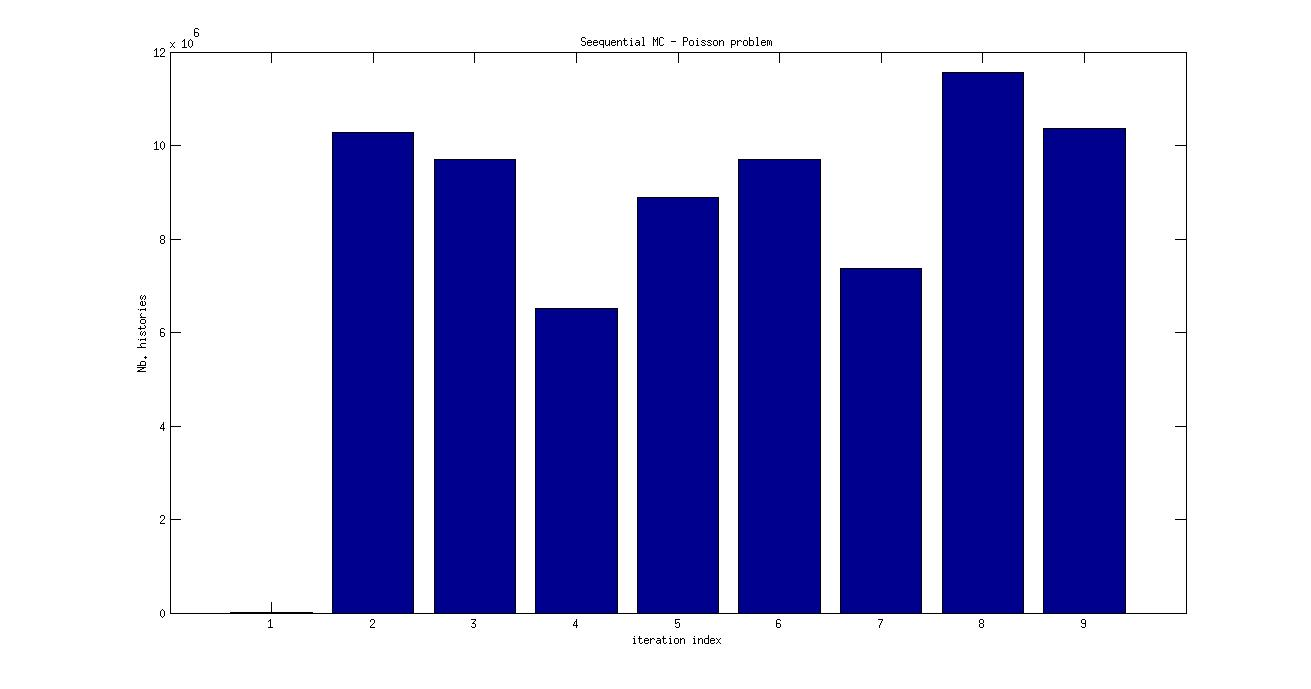
\includegraphics[width=\textwidth]{SEQ_poisson.eps}
\vspace{-0.3in}
    \caption{Sequential MC - Poisson problem. Number of random walks employed
at each iteration.}
\label{SEQ_poisson}
\end{figure}


\begin{figure}
  \centering
    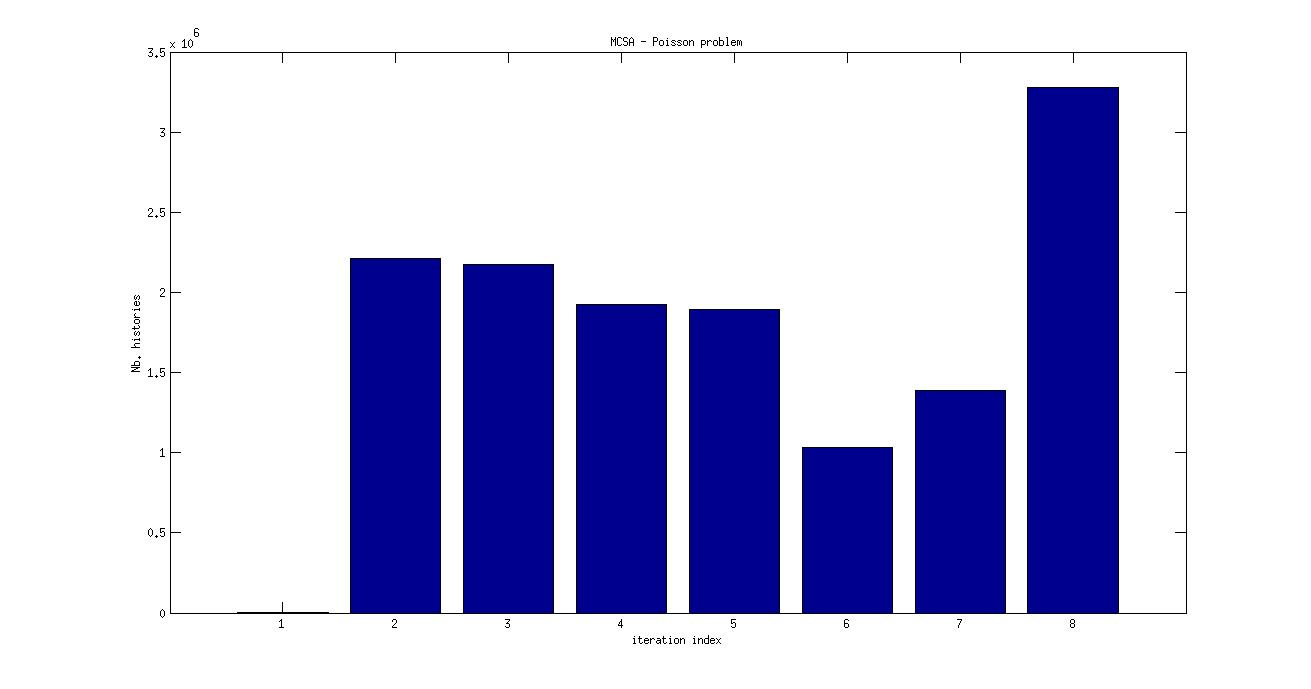
\includegraphics[width=\textwidth]{MCSA_poisson.eps}
\vspace{-0.3in}
      \caption{MCSA - Poisson problem. Number of random walks employed at each
iteration.}
\label{MCSA_poisson}
\end{figure}



\subsubsection{Reaction-diffusion problem}

Here we consider the simple reaction-diffusion problem

\begin{equation}
\begin{cases}
 -\Delta u +\sigma u= f \quad \text{in}\quad \Omega, \\
 u=0\quad \text{on} \quad \partial\Omega,
 \end{cases}
\end{equation}
where $\Omega=(0,1)\times (0,1)$, $\sigma=0.1$ and $f\equiv 1$.
A 5-point finite difference scheme is applied to discretize the problem.
The number of nodes
on each direction of the domain is 100, so that $h\approx 0.01$. The
discretized problem is $n\times n$ with $n=9604$. A left
diagonal preconditioning is again applied to
the coefficient matrix obtained from the discretization, which
is strictly diagonally dominant. The 1-norm of the
iteration matrix is $\lVert H\rVert_1\approx 0.9756$. This automatically
guarantees the convergence of the Adjoint Monte Carlo linear solver. 
In Table \ref{DR_results} a comparison between the deterministic
Richardson iteration, Sequential Monte Carlo and MCSA is provided.
The results are similar to those for the Poisson equation.
The number of histories per iteration for Sequential Monte Carlo and MCSA 
is shown in Figures \ref{SEQ_diffreac} and \ref{MCSA_diffreac}.

\begin{table}[!t]
\centering
\hspace*{-0.8cm}
\begin{tabular}{|c|c|c|c|}
\hline
algorithm & relative err.& \# iterations & average \# histories per iteration\\
\hline
 Richardson & $9.073\cdot 10^{-8}$ & 634 & - \\
\hline
 Sequential MC & $8.415 \cdot 10^{-8}$ &  8 & 12,391,375\\
 \hline
 Adjoint MCSA & $6.633 \cdot 10^{-8}$ &  7 & 3,163,700\\
\hline
\end{tabular}
\caption{Numerical results for the diffusion reaction problem.}
\label{DR_results}
\end{table}

\begin{figure}
  \centering
    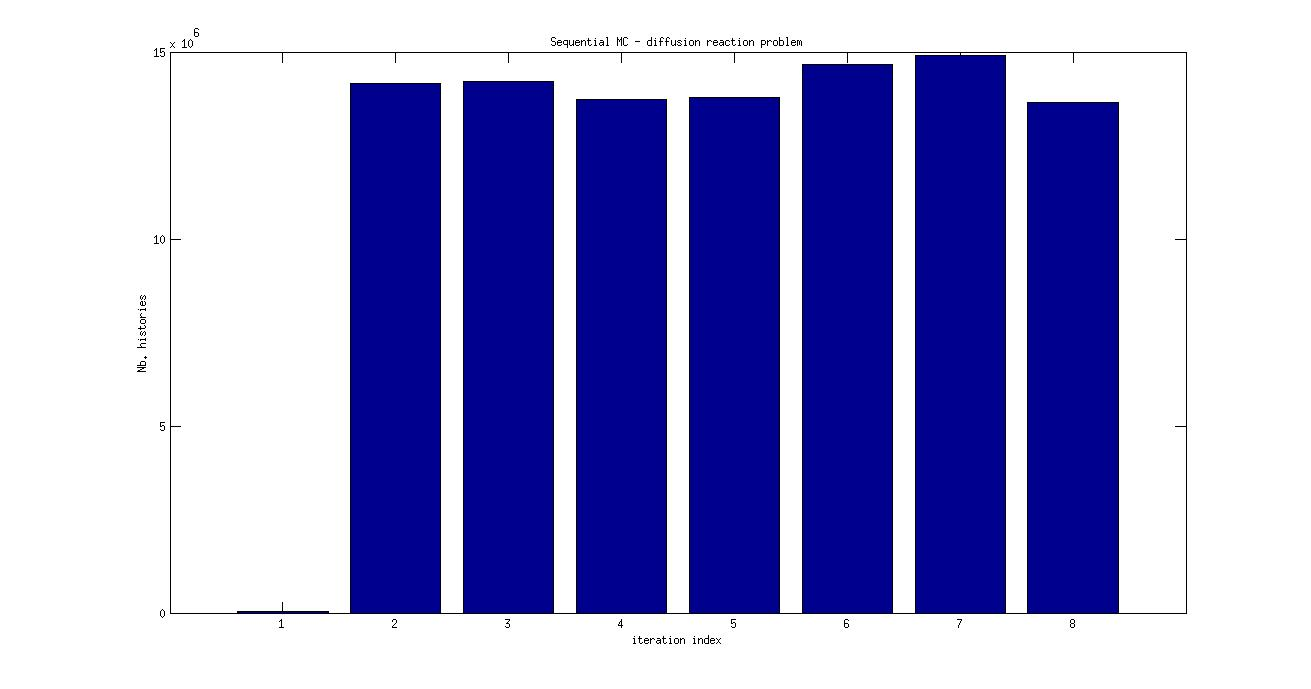
\includegraphics[width=\textwidth]{SEQ_diffreac.eps}
      \caption{Sequential MC - Reaction-diffusion problem. Number of random
walks
employed at each
 iteration.}
\label{SEQ_diffreac}
\end{figure}


\begin{figure}
  \centering
    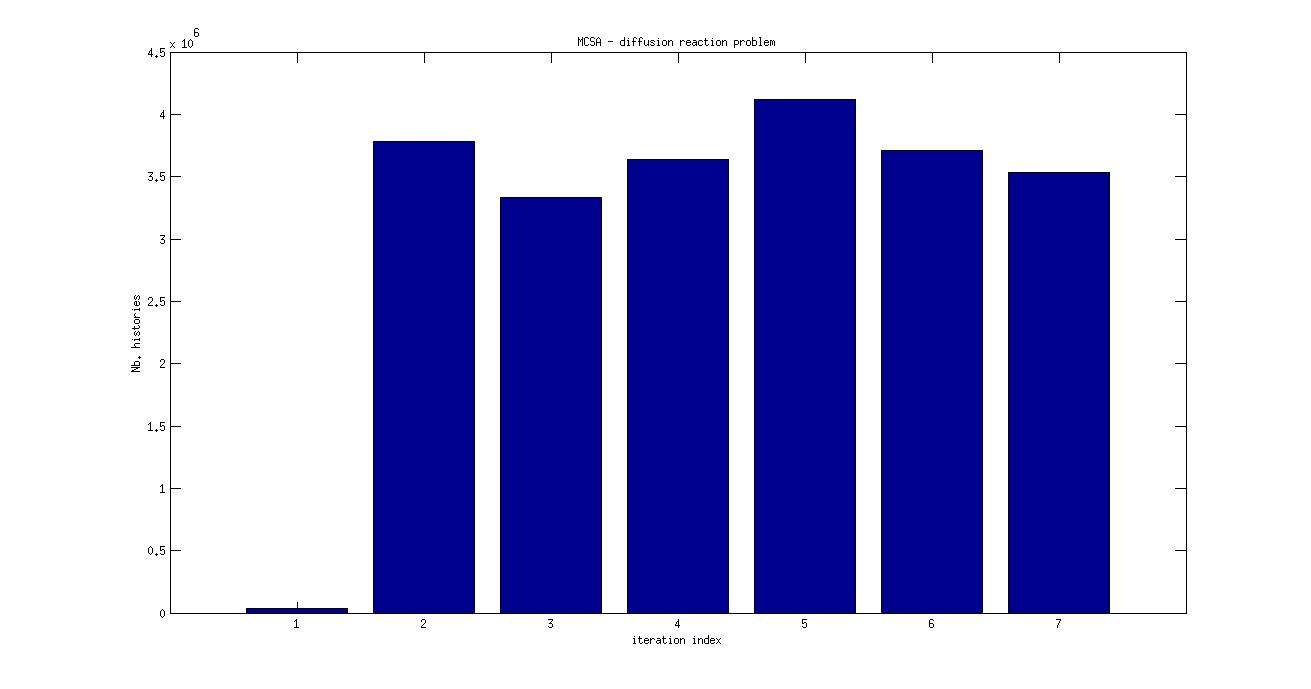
\includegraphics[width=\textwidth]{MCSA_diffreac.eps}
      \caption{MCSA - Reaction-diffusion problem. Number of random walks
employed at each
iteration.}
\label{MCSA_diffreac}
\end{figure}

\subsubsection{Parabolic problem}

Here we consider the 
following time-dependent problem:
\begin{equation}
 \begin{cases}\frac{\partial u}{\partial t} -\mu \Delta u
+\boldsymbol{\beta}(\mathbf{x})\cdot \nabla u=0, \;\; \quad \quad
\mathbf{x}\in \Omega,\quad t\in(0,T] \\
u(\mathbf{x},0) = u_0, \qquad \qquad \qquad \qquad \quad \mathbf{x}\in
\Omega \\
u(\mathbf{x},t)=u_D(\mathbf{x}),  \; \, \, \qquad \qquad \qquad \quad
\mathbf{x}\in \partial
\Omega, \quad t\in(0,T],
 \end{cases}
\end{equation}
where $\Omega = (0,1)\times (0,1)$, $T>0$,
$\mu=\frac{3}{200}$, $\boldsymbol{\beta}(\mathbf{x})=[2y(1-x^2),\;
-2x(1-y^2)]^T$, and $u_D=0$ on $\{\{x=0\}\times (0,1)\}$, $\{(0,1)\times
\{y=0\}\}$, $\{(0,1)\times \{y=1\}\}$.\newline

Implicit discretization in time (backward Euler scheme) with time step
$\Delta t$ and
a spatial discretization with quadrilateral linear finite elements using
the IFISS toolbox \cite{ifiss} leads
to a sequence of linear systems of the form
$$ \left (\frac{1}{\Delta t} M + A\right )\mathbf{u}^{k+1} = 
\mathbf{f}^k, \quad k=0,1,\ldots $$ 

Here we restrict our attention to a single generic time step.
The right-hand side is chosen so that the exact
solution to the linear system for the specific time step chosen is 
the vector of all ones. For the experiments we use a uniform discretization
with mesh size $h=2^{-8}$ and we let $\Delta t = 10h$.
The resulting linear system has $n=66,049$ unknowns.

We use the factorized
sparse approximate inverse AINV \cite{BT1998} as a right preconditioner,
with drop tolerance $\tau = 0.05$ for both inverse factors.
With this choice,
the spectral radius of the iteration matrix $H=I-AP^{-1}$ is $\rho(H)\approx
0.9218$ and the spectral radius of $\hat{H}$ for the Adjoint Monte Carlo is
$\rho(\hat{H})\approx 0.9148$. The MAO transition probability is employed.
 Resorting to a uniform probability in this case would have impeded
the
convergence, since in this case $\rho(\hat{H})\approx 1.8401$.
This is an example demonstrating how the MAO probability can 
improve the behavior of the stochastic algorithm, outperforming the
uniform one.

The fill-in ratio is given by $\frac{nnz(H)}{nnz(A)}=4.26$,
therefore the relative number of nonzero elements in $H$ is still acceptable
in terms of storage and computational costs.

As before,
the threshold for the check on the relative residual is set to $\varepsilon
=10^{-8}$, while the threshold
for the adaptive selection of the random walks is set
to $\varepsilon_1=0.1$.
The results for all three methods are shown in Table \ref{parabolic_results}. As 
one can see, both Sequential Monte Carlo and MCSA 
dramatically reduce the number of iterations with
respect to the purely deterministic
 preconditioned Richardson iteration, with MCSA oupterforming
Sequential Monte Carlo. 
Of course each iteration is now more expensive due to the Monte Carlo
calculations required at each Richardson iteration, but we stress
that Monte Carlo is an embarrassingly parallel method.
Monte Carlo calculations are also expected to be more robust in the
presence of faults, which is one of the main motivations for the
present work.

\begin{table}[!t]
\centering
\hspace*{-0.8cm}
\begin{tabular}{|c|c|c|c|}
\hline
algorithm & relative err.& \# iterations & average \# histories per iteration\\
\hline
 Richardson & $6.277\cdot 10^{-7}$ & 178 & - \\
 \hline
 Sequential MC & $1.918 \cdot 10^{-9}$ & 8 & 51,535,375\\
\hline
 Adjoint MCSA & $1.341\cdot 10^{-9}$ & 6 & 16,244,000\\
\hline
\end{tabular}
\caption{Numerical results for the parabolic problem.}
\label{parabolic_results}
\end{table}


\begin{figure}
  \centering
    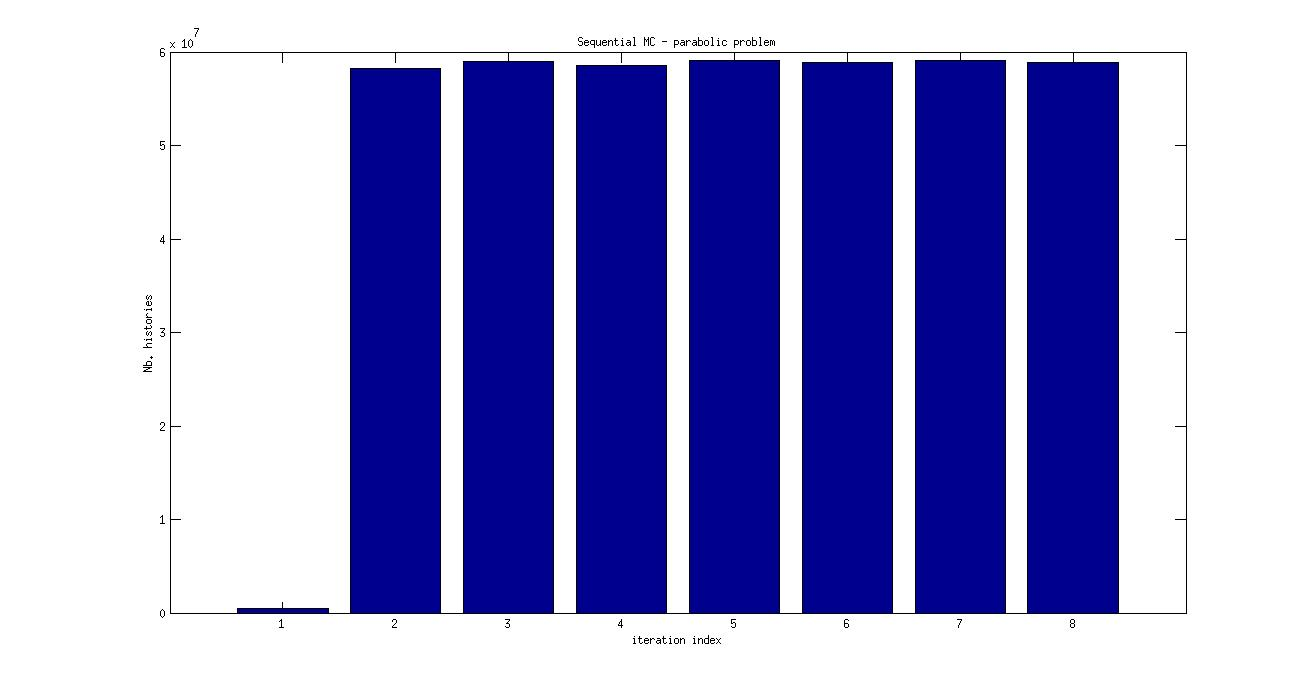
\includegraphics[width=\textwidth]{SEQ_parabolic.eps}
      \caption{Sequential Monte Carlo - Parabolic problem. Number of random
walks
employed at each
iteration.}
\label{SEQ_parabolic}
\end{figure}


\begin{figure}
  \centering
    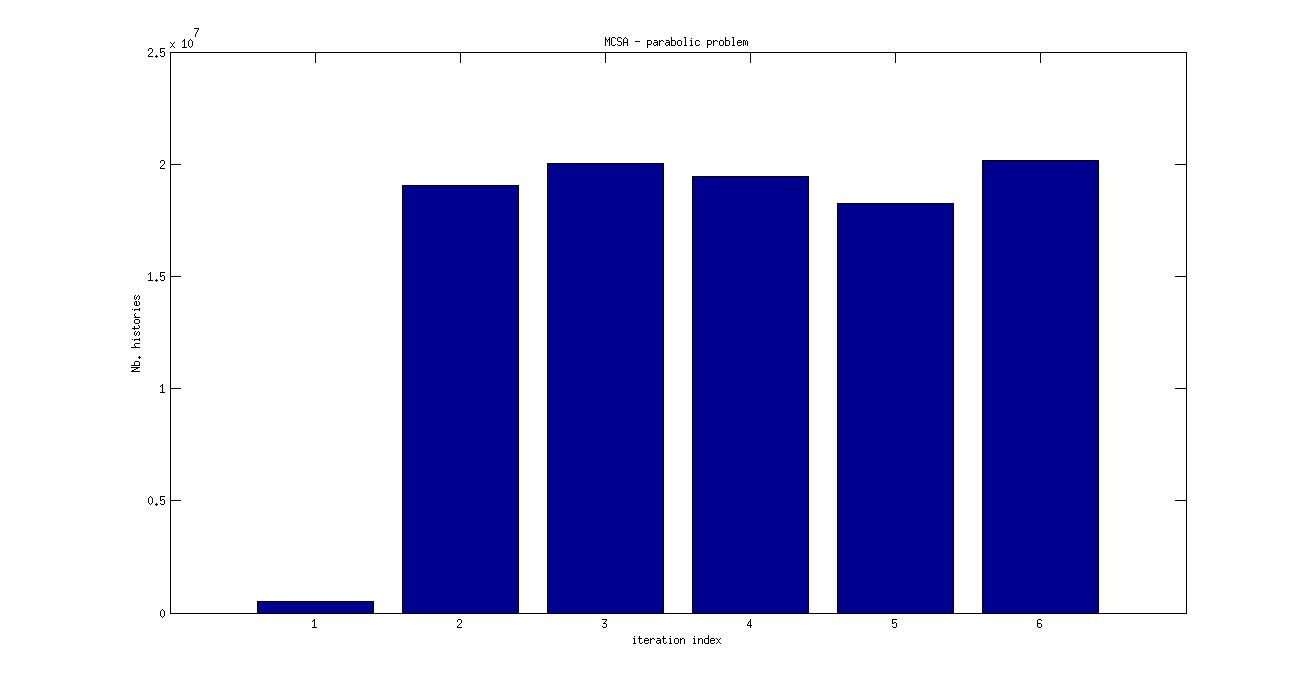
\includegraphics[width=\textwidth]{MCSA_parabolic.eps}
      \caption{MCSA - Parabolic problem. Number of random walks
employed at each
iteration.}
\label{MCSA_parabolic}
\end{figure}

Finally, Figures \ref{SEQ_parabolic} and \ref{MCSA_parabolic} 
show the number of Monte Carlo histories per iteration 
for Sequential Monte Carlo
and for MCSA, respectively.

\section{Conclusions and future work}
\label{sec:conclusion}

In this paper we have reviewed known convergence conditions for Monte Carlo linear
solvers and established a few new sufficient conditions. In particular, we
have determined classes of matrices for which the method  is guaranteed
to converge. The main focus has
been on the recently proposed MCSA algorithm, which clearly outperforms
previous approaches. This method combines a deterministic fixed point
iteration (preconditioned Richardson method) with a Monte Carlo 
acceleration scheme, typically an Adjoint Monte Carlo estimator. Various
types of preconditioners have been tested, including diagonal, block
diagonal, and sparse approximate inverse preconditioning.  

Generally speaking, it is difficult to ensure a priori that the
hybrid solver will converge. In particular, convergence of the underlying
preconditioned Richardson iteration is necessary, but not sufficient. 
The application of hybrid solvers to non-diagonally dominant, steady-state
problems presents a challenge and may require some trial-and-error in the
choice of tuning parameters, such as the block size or drop tolerances; 
convergence can be guaranteed for some standard model problems but in 
general it is difficult to enforce.
This is an inherent limitation of hybrid deterministic-stochastic
approaches of the kind considered in this paper.

On a positive note, numerical experiments show that these methods 
are quite promising for solving strictly diagonally dominant linear systems 
arising from time-dependent simulations, such as unsteady diffusion and
advection-diffusion type equations. Problems of this type are quite
important in practice, as they are often the most time-consuming part
of many large-scale CFD and radiation transport simulations. 
Linear systems with such properties also arise in other application areas,
such as network science and data mining.

In this paper we have not attempted to analyze the algorithmic scalability 
of the hybrid solvers. A difficulty is the fact that these methods contain
a number of tuneable parameters, each one of which can have great impact on 
performance and convergence behavior:
the choice of preconditioner, the stopping
criteria used for the Richardson iteration, the criteria for the number
and length of Monte Carlo histories to be run at each iteration, the 
particular estimator used, and
possibly others. While the cost per iteration is linear in the
number $n$ of unknowns, it is not clear how to predict the rate of convergence of
the outer iterations, since it depends strongly on the amount of work
done in the Monte Carlo acceleration phase, which is also not known a
priori except for some rather conservative upper bounds. Clearly,
the scaling behavior of hybrid methods with respect to problem size
needs to be further investigated.

Future work should also focus on testing hybrid methods on 
large parallel architectures and on evaluating their resiliency in the presence
of simulated faults. Efforts in this direction are currently under way. 

\section*{Acknowledgments}
We are indebted to Miroslav T\accent23 uma for help with the AINV code used
in some of the numerical experiments.



\begin{thebibliography}{9}

  \bibitem{Agullo}
  {\sc E.~Agullo, L.~Giraud, A.~Guermouche, J.~Roman, and M.~Zounon},
  {\em Towards resilient parallel linear Krylov solvers: recover-restart
  strategies},
  Research Report N. 8324, June 2013, Project-Teams HiePACS, INRIA.
 
 \bibitem{AADBTW2005}
 {\sc V.~Alexandrov, E.~Atanassov, I.~T.~Dimov, S.~Branford, A.~Thandavan, and 
C.~Weihrauch},
{\em Parallel hybrid Monte Carlo algorithms for matrix computations 
problems},
Lecture Notes in Computer Science,
3516 (2005), pp.~752--759.
 
 \bibitem{Ax1994}
 {\sc O.~Axelsson},
 {\em Iterative Solution Methods},
 Cambridge University Press, 1994. 
 
 \bibitem{Benzi2002}
 {\sc M.~Benzi}, 
 {\em Preconditioning techniques for large linear systems: a survey},
 Journal of Computational Physics,
 182 (2002), pp.~417--477.

 \bibitem{BMT1996}
 {\sc M.~Benzi, C.~D.~Meyer, and M.~Tuma},
 {\em A sparse approximate inverse preconditioner for the 
 conjugate gradient method},
  SIAM Journal on Scientific Computing,
  17 (1996), pp.~1135--1149.

 \bibitem{BT1998}
 {\sc M.~Benzi and M.~T\accent23uma},
 {\em A sparse approximate inverse preconditioner for nonsymmetric linear 
systems},
  SIAM Journal on Scientific Computing,
  19 (1998), pp.~968--994.

\bibitem{BP1979}
{\sc A.~Berman and R.~J.~Plemmons},
{\em Nonnegative Matrices in the Mathematical Sciences}, 
Academic Press, New York, 1979.

\bibitem{CFL}
{\sc R.~Courant, K.~Friedrichs, and H.~Lewy},
{\em \"Uber die partiellen Differenzengleichungen der mathematischen
Physik}, Mathematische Annalen, 100 (1928), pp.~32--74.

\bibitem{Curtiss}
{\sc J.~H.~Curtiss},
{\em Sampling methods applied to differential and difference equations},
Proc.~Seminar on Scientific Computation, Nov.~1949, IBM, New York, 1950, pp.~87--109. 

 \bibitem{DA1998}
 {\sc I.~T.~Dimov and V.~N.~Alexandrov}, 
 {\em A new highly convergent Monte Carlo method for matrix computations},
 Mathematics and Computers in Simulation, 
 47 (1998), pp.~165--181.
 
 \bibitem{DVA2001}
 {\sc I.~T.~Dimov, V.~Alexandrov, and A.~Karaivanova},
 {\em Parallel resolvent Monte Carlo algorithms for linear algebra 
 problems},
 Mathematics and Computers in Simulation,
 55 (2001), pp.~25--35.

\bibitem{ifiss}
{\sc H.~C.~Elman, A.~Ramage, and D.~J.~Silvester}, 
{\em IFISS: A computational laboratory for investigating incompressible flow problems},
 SIAM Review, 56 (2014), pp.~261--273.
 
 \bibitem{EMSH2014}
 {\sc T.~M.~Evans, S.~W.~Mosher, S.~R.~Slattery, and S.~P.~Hamilton},
 {\em A Monte Carlo synthetic-acceleration method for solving the thermal 
 radiation diffusion equation},
 Journal of Computational Physics, 
 258 (2014), pp.~338--358.
 
 \bibitem{ESW2013}
 {\sc T.~M.~Evans, S.~R.~Slattery, and P.~P.~H.~Wilson}, 
 {\em A spectral analysis of the domain decomposed Monte Carlo method for 
linear systems},
 International Conference on Mathematics and Computational Methods 
Applied to Nuclear Science \& Engineering, 2013.

\bibitem{FLRU15}
 {\sc M.~Fasi, J.~Langou, Y.~Robert, and B.~U\c car},
 {\em A backward/forward recovery approach for the preconditioned
  conjugate gradient method}, arXiv:1511.04478v1, 13 November 2015.

\bibitem{FV62}
{\sc D.~F.~Feingold and R.~S.~Varga},
  {\em Block diagonally dominant matrices and generalizations
   of the Gerschgorin circle theorem},
Pacific Journal of Mathematics, 4 (1962), pp.~1241--1250.
 
\bibitem{FL50}
{\sc G.~E.~Forsythe and R.~A.~Leibler},
{\em Matrix inversion by a Monte Carlo method},
Math.~Tables Other Aids Comput., 6 (1952), pp.~78--81. 
  
  \bibitem{FK1975}
  {\sc S.~Friedland and S.~Karlin},
  {\em Some inequalities for the spectral radius of non-negative matrices 
  and applications},
  Duke Mathematical Journal, 
  42 (1975), pp.~459--490.

 \bibitem{Hal1962}
 {\sc J.~H.~Halton},
 {\em Sequential Monte Carlo},
 Mathematical Proceeding of the Cambridge Philosophical Society,
 58 (1962), pp.~57--58.
 
 \bibitem{Hal1994}
 {\sc J.~H.~Halton}, 
 {\em Sequential Monte Carlo techniques for the solution of linear 
systems},
 Journal of Scientific Computing,
 9 (1994), pp.~213--257.
 
 \bibitem{MASC2013}
 {\sc J.~Hao, M.~Mascagni, and Y.~Li},
 {\em Convergence analysis of Markov chain Monte Carlo linear solvers using 
Ulam-von Neumann algorithm},
 SIAM Journal on Numerical Analysis,
 51 (2013), pp.~2107--2122.

  \bibitem{Heroux}
  {\sc M.~Hoemmen and M.~Heroux},
  {\em Fault-tolerant iterative methods via selective reliability},
  Proceedings of the 2011 International Conference for High Performance
Computing, Networking, Storage and Analysis (SC), vol.~3, IEEE Computer Society,
2011.
  
  \bibitem{Horn1994}
  {\sc R.~A.~Horn and C.~R.~Johnson},
  {\em Topics in Matrix Analysis},
  Cambridge University Press, 1994.
 
  \bibitem{Li2002}
  {\sc L.~Li},
  {\em On the iterative criterion for generalized diagonally dominant 
matrices},
  SIAM Journal on Matrix Analysis and Applications,
  24 (2002), pp.~17--24.
 
 \bibitem{Saad}
 {\sc Y.~Saad}, 
 {\em Iterative Methods for Sparse Linear Systems},
 Society for Industrial and Applied Mathematics, Philadelphia, 2003.
  
  \bibitem{Rizzi}
  {\sc K.~Sargsyan, F.~Rizzi, P.~Mycek, C.~Safta, K.~Morris, H.~Najm,
  O.~Le Maitre, O.~Knio, and B.~Debusschere},
  {\em Fault resilient domain decomposition preconditioner for PDEs},
  SIAM Journal on Scientific Computing,
  37 (2015), pp.~A2317--A2345.
 
 \bibitem{Slattery2013}
 {\sc S.~Slattery},
 {\em Parallel Monte Carlo Synthetic Acceleration Methods For Discrete 
Transport Problems},
 Ph.D.~Thesis, University of Wisconsin-Madison, 2013.
 
 \bibitem{Srin2010}
 {\sc A.~Srinivasan}, 
 {\em Monte Carlo linear solvers with non-diagonal splitting},
 Mathematics and Computer in Simulation,
 80 (2010), pp. 1133-1143.

 \bibitem{Stoyanov}
 {\sc M.~Stoyanov and C.~Webster},
 {\em Numerical analysis of fixed point algorithms in the presence of hardware
  faults},
  SIAM Journal on Scientific Computing,
  37 (2015), pp.~C532--C553.
 
\end{thebibliography}


\end{document}
